% This LaTeX document needs to be compiled with XeLaTeX.
\documentclass[
  10
]{article}
\usepackage[margin=2cm,includehead=true,includefoot=true,centering,]{geometry}
\usepackage{xcolor}
\usepackage{ucharclasses}
\usepackage{xurl}
\usepackage{hyperref}
\usepackage{amsmath,amssymb}
\usepackage{amsfonts}
\usepackage[version=4]{mhchem}
\usepackage{stmaryrd}
\usepackage{bbold}
\usepackage{polyglossia}
\usepackage{fontspec}
\usepackage{ctex}
\usepackage[export]{adjustbox}
\usepackage{tabularx}
\usepackage{booktabs}

\usepackage{setspace}
\setstretch{1.2}

\makeatletter
\@ifundefined{KOMAClassName}{% if non-KOMA class
  \IfFileExists{parskip.sty}{%
    \usepackage{parskip}
  }{% else
    \setlength{\parindent}{0pt}
    \setlength{\parskip}{6pt plus 2pt minus 1pt}}
}{% if KOMA class
  \KOMAoptions{parskip=half}}
\makeatother
\usepackage{longtable,booktabs,array}
\newcounter{none} % for unnumbered tables
\usepackage{multirow}
\usepackage{calc} % for calculating minipage widths
% Correct order of tables after \paragraph or \subparagraph
\usepackage{etoolbox}
\makeatletter
\patchcmd\longtable{\par}{\if@noskipsec\mbox{}\fi\par}{}{}
\makeatother
% Allow footnotes in longtable head/foot
\IfFileExists{footnotehyper.sty}{\usepackage{footnotehyper}}{\usepackage{footnote}}
\makesavenoteenv{longtable}
\usepackage{graphicx}
\makeatletter
\newsavebox\pandoc@box
\newcommand*\pandocbounded[1]{% scales image to fit in text height/width
  \sbox\pandoc@box{#1}%
  \Gscale@div\@tempa{\textheight}{\dimexpr\ht\pandoc@box+\dp\pandoc@box\relax}%
  \Gscale@div\@tempb{\linewidth}{\wd\pandoc@box}%
  \ifdim\@tempb\p@<\@tempa\p@\let\@tempa\@tempb\fi% select the smaller of both
  \ifdim\@tempa\p@<\p@\scalebox{\@tempa}{\usebox\pandoc@box}%
  \else\usebox{\pandoc@box}%
  \fi%
}
% Set default figure placement to htbp
\def\fps@figure{htbp}
\makeatother
\setlength{\emergencystretch}{3em} % prevent overfull lines
\providecommand{\tightlist}{%
  \setlength{\itemsep}{0pt}\setlength{\parskip}{0pt}}


\hypersetup{colorlinks=true, linkcolor=blue, filecolor=magenta, urlcolor=cyan,}
\urlstyle{same}

\usepackage{colortbl}
\definecolor{table-row-color}{HTML}{999999}
\definecolor{table-rule-color}{HTML}{999999}
%\arrayrulecolor{black!40}
\arrayrulecolor{table-rule-color}     % color of \toprule, \midrule, \bottomrule
\setlength{\aboverulesep}{0pt}
\setlength{\belowrulesep}{0pt}


\setotherlanguages{english}
\IfFontExistsTF{Songti SC}
{\newfontfamily\chinesefont{Songti SC}}
{\IfFontExistsTF{Source Han Serif CN}
{\newfontfamily\chinesefont{Source Han Serif CN}}
{\IfFontExistsTF{Noto Serif CJK SC}
  {\newfontfamily\chinesefont{Noto Serif CJK SC}}
  {\IfFontExistsTF{SimSun}
    {\newfontfamily\chinesefont{SimSun}}
    {\IfFontExistsTF{FangSong}
      {\newfontfamily\chinesefont{FangSong}}
      {\newfontfamily\chinesefont{Arial Unicode MS}}
}}}}
\setCJKmainfont{Songti SC}
\setCJKsansfont{Heiti SC}

\IfFontExistsTF{Times New Roman}
{\newfontfamily\englishfont{Times New Roman}}
{\IfFontExistsTF{Liberation Serif}
  {\newfontfamily\englishfont{Liberation Serif}}
  {\IfFontExistsTF{DejaVu Serif}
    {\newfontfamily\englishfont{DejaVu Serif}}
    {\newfontfamily\englishfont{Arial}}
}}


\usepackage{ragged2e}
\newcolumntype{L}[1]{>{\RaggedRight\arraybackslash}p{#1}}
\newcolumntype{C}[1]{>{\Centering\arraybackslash}p{#1}}
\setlength{\LTcapwidth}{\textwidth}
\usepackage{caption}
\captionsetup{labelfont=bf, labelsep=quad, justification=raggedright,
              singlelinecheck=false}

\author{}
\date{}

\begin{document}

\renewcommand{\figurename}{图}
\renewcommand{\tablename}{表}


\begin{center}

\includegraphics[width=0.34\linewidth]{images_hi/title_logo.png}
\vspace{1.0em}

{\LARGE MiMo-V2.6: Scaling Reinforcement Learning\\[0.25em] Towards Self-Improvement\par}
\vspace{0.5em}
{\large MiMo-V2.6：面向自我改进的强化学习扩展\par}
\vspace{0.8em}
{\normalsize LLM-Core Xiaomi\par}
\end{center}

\renewcommand{\contentsname}{目录}
\tableofcontents
\clearpage

\section*{摘要}\label{abstract}

强化学习（RL）是推动大型基础模型走向自我改进的核心训练范式。本报告
介绍 MiMo-V2.6 系列，这是一个通过扩展 RL 算力推动模型智能前沿的全模态
家族。在 RL 之前，我们在广泛的多模态语料上进行中期训练，以提供充足的
探索空间，并在预训练的混合 SWA 架构上构建扎实的基础设施以支撑后续的
规模扩展。我们从三个维度扩展 RL 算力：（1）更大的批大小与更高的
吞吐，采用异步训练，每步消耗 1,568 个样本和 $2.7\sim$3.7B tokens，上下文
长度最高 1M；（2）更多样、更复杂的环境，在多种智能体脚手架的组合下
覆盖代码、通用、视觉和网络安全领域；（3）更多评分器算力，通过组内
智能体评分，为长程任务产出更准确的奖励信号，并引导模型走向更短、
更省 token 的解法。为在规模扩展下保持训练稳定，我们冻结 MoE 路由器，
并建立针对奖励作弊的多层防御。我们进一步构建混合任务智能体 RL 的
基础设施，包括统一的轨迹表示、高并发多框架 rollout、控制面与数据面
解耦，以及训练与推理的一致性。我们开源了训练动态、RL 环境和 RL 框架，
以促进复现以及关于规模化 RL 与模型自我改进的后续研究。







\begin{figure}[htbp]
\centering
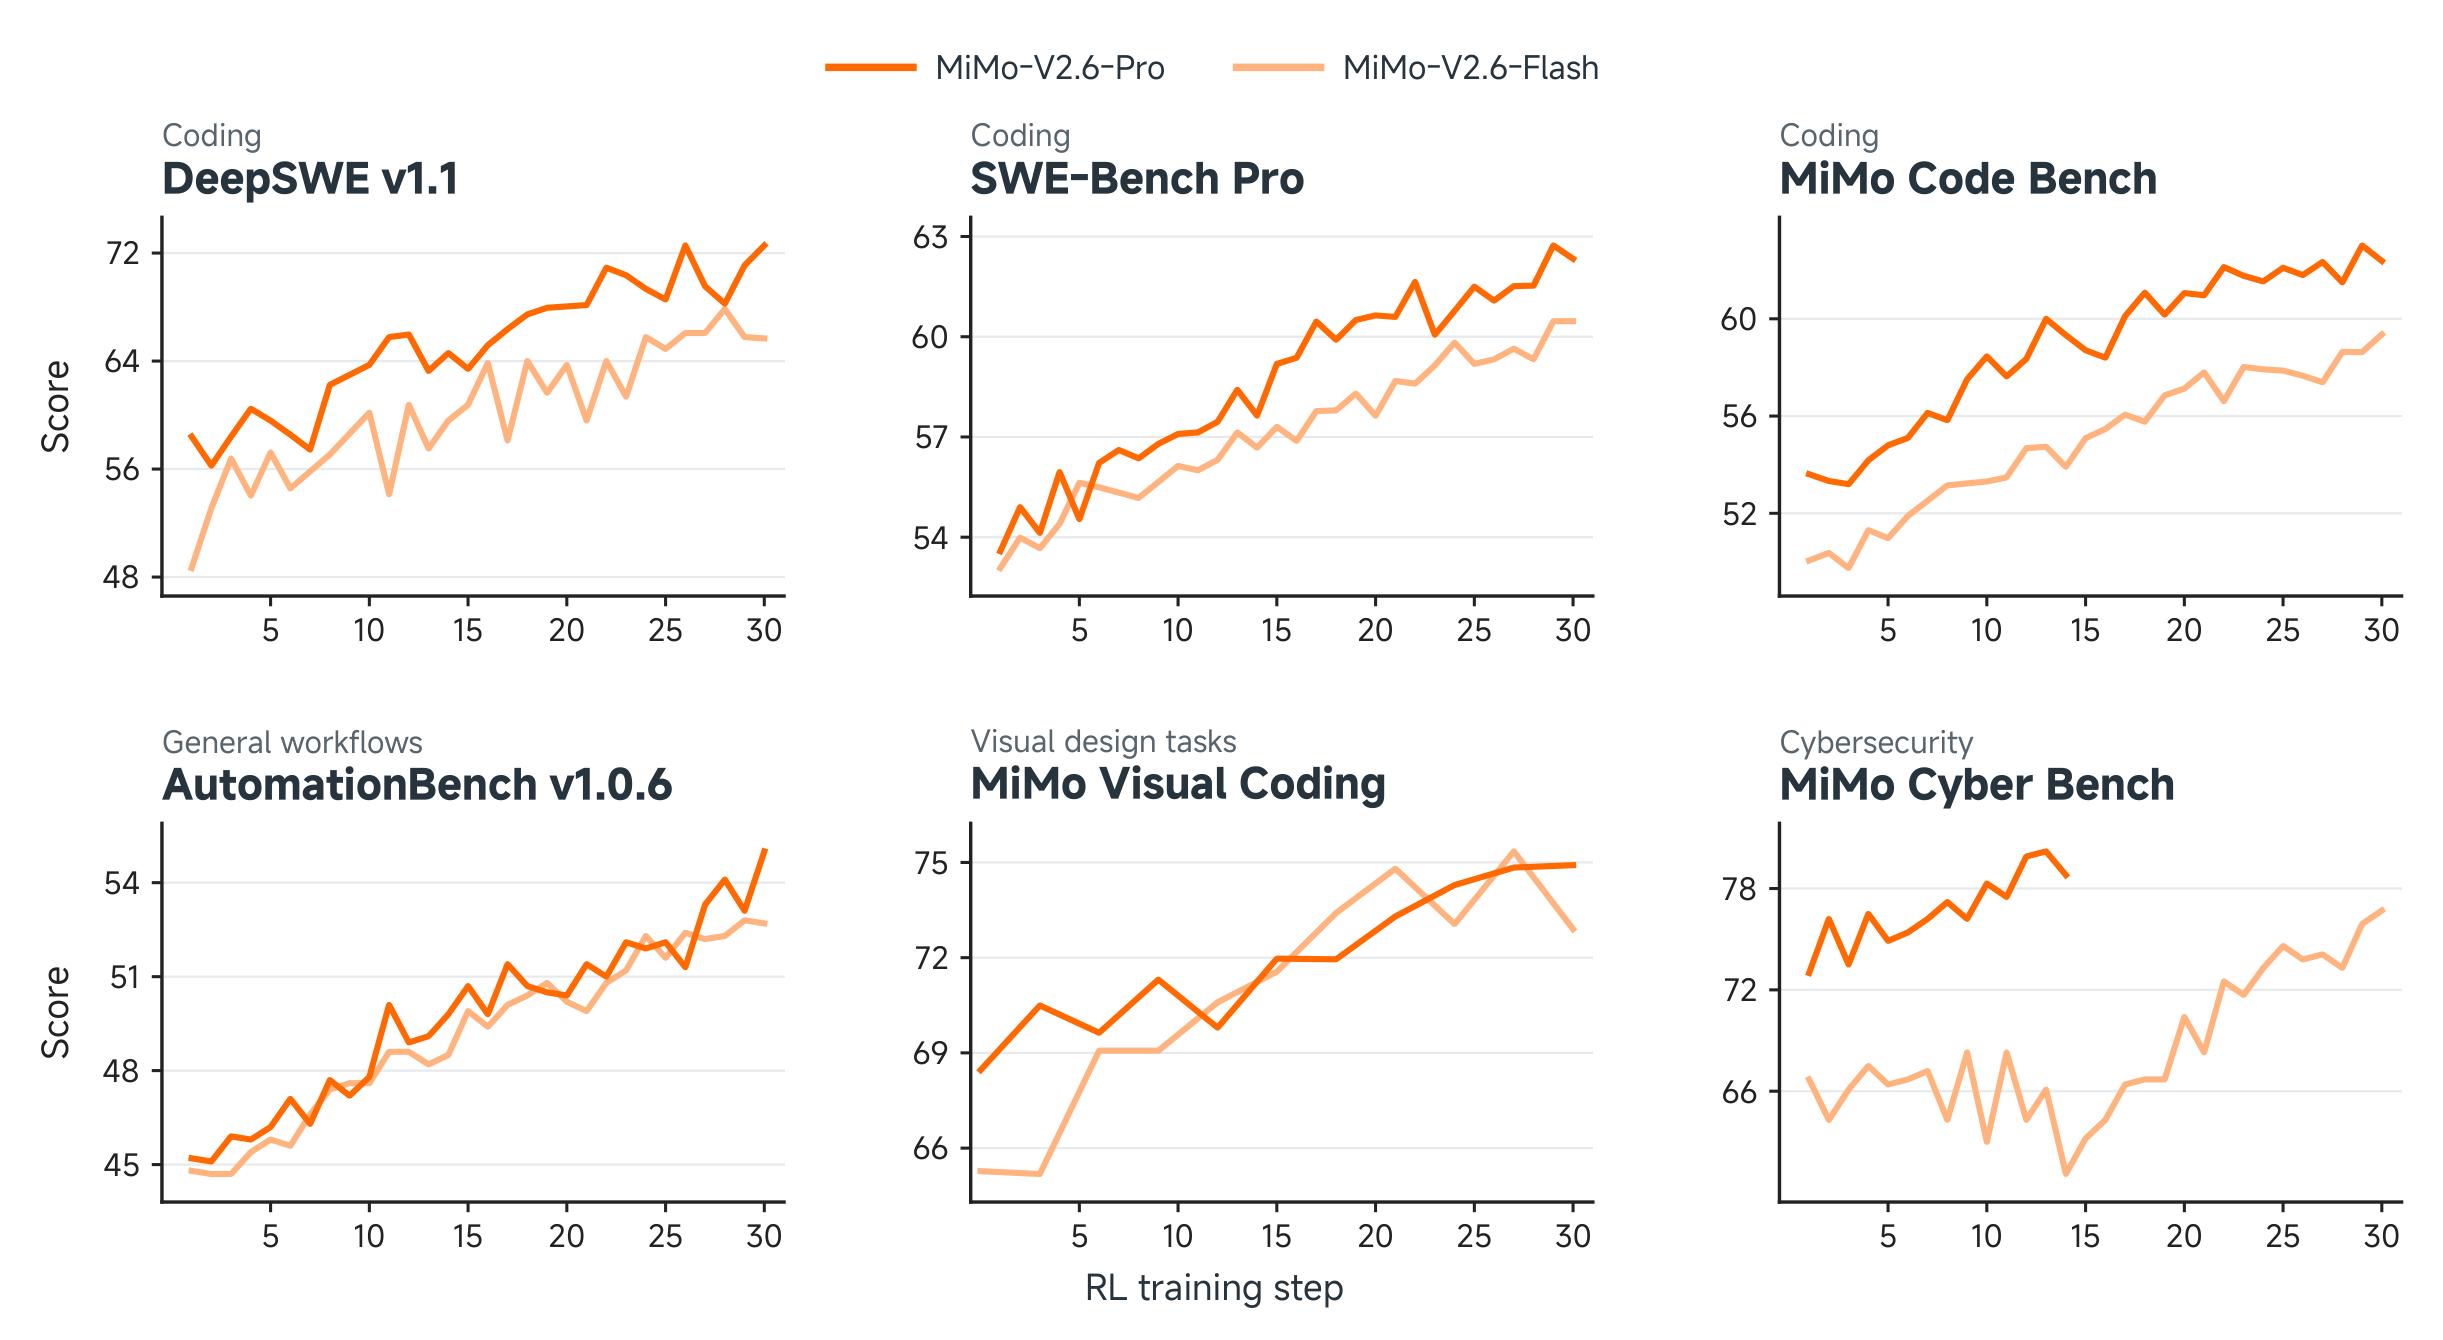
\includegraphics[width=\linewidth]{images_hi/fig01.png}
\caption{MiMo-V2.6-Pro 与 MiMo-V2.6-Flash 在整个 RL 训练过程中各任务的基准得分。}
\label{fig:1}
\end{figure}


\section{引言}\label{introduction}

递归自我改进（RSI）设想模型通过持续的探索与反馈来扩展自身能力。
实现这一愿景需要智能体，它们把模型与交互式环境耦合起来，从而提供
自我改进所依赖的多步轨迹和反馈信号。为此，在复杂的智能体任务上
扩展强化学习（RL）开辟了一条具体的路径。然而，释放这一潜力面临两大
挑战。第一，面向基础模型的 RL 需要合适的模型架构，以及为智能体提供
足够丰富的探索空间。第二，扩展 RL 需要基础设施、环境和评分器方面的
成熟方案。在本报告中，我们介绍 MiMo-V2.6 系列，包括 MiMo-V2.6-Pro——
一个 1.02T 参数、42B 激活参数的专家混合（MoE）模型，以及
MiMo-V2.6-Flash——一个 310B 参数、15B 激活参数的专家混合（MoE）模型，
以弥合这些差距，在规模化 RL 上迈出务实的一步。

MiMo-V2.6 的架构、预训练和中期训练共同构建了一个强大且高效的基础
模型。出于以低计算成本保留全局上下文的需要，MiMo-V2.6 构建了混合
稀疏 MoE Transformer 主干，将局部滑动窗口注意力（SWA）与全局注意力
（GA）交错排布，并辅以轻量视觉编码器和音频编码器。此外，大规模
预训练赋予模型广泛的知识，以及在文本、音频和视频上的多模态理解能力。
我们进一步引入以智能体为中心的中期训练阶段，扩展智能体任务的探索
空间，使模型在后训练期间能够发现更有效的解题轨迹。

接下来，我们通过一个系统化、协同设计的框架在三个关键组件上扩展 RL
算力。第一，我们通过全异步训练扩展批大小和训练吞吐，每步处理数千条
长程 rollout 和数十亿 token，上下文长度最高 1M。第二，我们扩展 RL
环境的多样性和复杂度，覆盖编码、通用、视觉和网络安全任务，使用
多样化的智能体脚手架，并加强对奖励作弊的防护。同时变化脚手架和任务
可以提升模型的泛化能力。第三，我们引入组内智能体评分，在二元测试
用例之外提供信息量更大的奖励信号。我们不再给所有通过测试用例的解法
分配相同奖励，而是在每个组内比较各解法，以区分解题质量和行为。通过
我们提出的组内奖励合成（GRS）和组内优势重分配（GAR），这些细粒度的
区分被转化为信息量更大的学习信号，引导模型走向更准确、更高效的解法。

在规模化实现这些，需要基础设施在研究和工程两方面应对挑战。为支持
灵活的智能体交互场景，我们设计了统一的轨迹表示和惩罚机制，二者共同
精炼学习信号。为处理大训练批，我们通过脚手架池在多种智能体框架间
维持高并发交互，并将控制面与数据面解耦，以缓冲和传输携带路由与
多模态负载的海量轨迹。样本混合机制与动态采样和部分 rollout 协同工作，
稳定训练批中每个任务的样本组成。我们在 MoE 路由和 top-p 采样的候选
集合上对齐训练与推理引擎，并针对 RL 负载优化两个引擎。

扩展 RL 算力显著释放了模型在可验证任务（如编码）和较难验证任务
（如网页开发）上的潜力。如图 1 所示，随着训练步数增加，MiMo-V2.6-Pro
和 MiMo-V2.6-Flash 在所报告的基准上均稳步提升。而且这些收益并不局限
于单一领域，而是在多样任务上一致成立，涵盖 DeepSWE
（Huang et al., 2026）上的编码、AutomationBench
（Shepard and Salimans, 2026）上的通用工作流、MiMo Visual Coding 上的
视觉任务，以及 MiMo Cyber Bench 上的网络安全。这些收益表明，
MiMo-V2.6 具备更强的复杂问题求解能力，在日常协同工作场景中表现更
可靠，体现出更通用的智能体智能。

为促进智能体 RL 的研究，我们开源了一套覆盖 RL 开发栈关键组件的综合
套件，包括轻量模型 MiMo-V2.6-Distill-Qwen-9B、带校验器的多领域精选
任务环境、端到端 RL 训练框架，以及用于灵活智能体交互的可组合
mini-harness。这些组件共同为在多样任务、环境和智能体配置下研究智能体
RL 提供了统一且易用的平台，同时降低了复现和扩展大规模 RL 实验的工程
门槛。在 MiMo-V2.6-Distill-Qwen-9B 上的实验表明，RL 在多样任务和智能体
脚手架上均带来一致的收益，验证了所提套件的有效性和通用性。我们希望
这套开源套件能成为社区公平、强大且可复现的基线，支持对智能体 RL 的
系统性研究，并推动面向递归自我改进的研究。

\section{架构}\label{architecture}

\subsection{整体架构}\label{overall-architecture}

如图 2 所示，MiMo-V2.6 采用标准 Transformer（Vaswani et al., 2017）
主干，并辅以通过轻量投影器连接的视觉编码器和音频编码器。

MiMo-V2.6 的文本主干主要由重复的混合块组成，这些块将局部滑动窗口
注意力（SWA）与全局注意力（GA）交错排布。它堆叠 $M$ 个混合块，每个
块由 $N$ 个连续的 SWA 块后接一个 GA 块构成。唯一的例外是最开始的
Transformer 块，它使用带稠密前馈网络（FFN）的全局注意力，以稳定早期的
表示学习。MiMo-V2.6 中使用的滑动窗口大小 $W$ 为 128。SWA 块和 GA 块
都使用不带共享专家的稀疏 MoE FFN。MiMo-V2.6 还集成了基于 SWA 和稠密
FFN 的 MTP（Gloeckle et al., 2024; Liu et al., 2024; Xia et al., 2025），
以在预训练期间提升模型性能。关于文本主干架构更全面的描述可参见
Core Team et al.~(2026)。模型配置见表 1。

\subsection{MiMo-ViT}\label{mimo-vit}

MiMo-ViT 采用混合注意力架构。它将 MiMo-VL-7B（Yue et al., 2025）中固定、不重叠的窗口注意力替换为带 sink 增强的 SWA，使信息能够在相邻层之间跨窗口边界交换，缓解视觉碎片化。局部 SWA 层在行优先与列优先的 token 序列化之间交替，以支持信息沿两个空间轴传播。此外，GA 层被周期性地插入，以直接聚合全局上下文。该设计大幅降低了高分辨率视觉处理的计算开销，同时达到与 GA ViT 相当的性能。更多分析请参见 He et al.~(2026)。为从零预训练 MiMo-ViT，我们将其与一个小规模预训练 LLM 配对，仅在多模态理解数据上以交叉熵目标优化所得的 VLM。这一简单配方避免了对比学习等辅助目标，使预训练高效且可扩展。关键在于，LLM 保持可训练，从而为 ViT 提供稳定且语义有意义的梯度。在超过 4T 图像 token 上预训练后，MiMo-ViT 学到了强视觉表征，可作为 MiMo-V2.6 的稳健基础。




\begin{figure}[htbp]
\centering

\includegraphics[width=\linewidth]{images_hi/fig02.png}
\caption{MiMo-V2.6 的整体架构。音频、视觉与文本输入被映射为共享的 token 序列，由 MiMo 混合 SWA 主干处理，随后经过语言建模头和多 token 预测（MTP）块。}
\label{fig:2}
\end{figure}

\subsection{音频编码器}\label{audio-encoder}

MiMo-V2.6 中的音频编码分为两个阶段：先用 Audio Tokenizer 进行音频分词，随后进行 patch 编码。Audio Tokenizer 编码器首先通过两层卷积前端处理 log-mel 频谱图，将帧率减半。得到的序列随后经过一个 Transformer，其因果混合注意力架构交替堆叠 SWA 与 GA 层。SWA 层捕捉局部时间依赖，GA 层则在完整的前序序列上聚合上下文。随后的下采样卷积将帧率进一步减半至 25 Hz，之后一个 20 层残差向量量化器（RVQ）将每一帧表示为 20 个离散音频 token。Audio Tokenizer 沿用 MiMo-Audio（Xiaomi, 2025）的训练配方，在涵盖语音、音乐及其他音频内容的 2000 万小时音频上训练。

音频 patch 编码器沿用 MiMo-Audio 的架构设计，并与文本主干联合训练。在每个时间步，音频 token 通过各自独立的嵌入表进行嵌入，每个 RVQ 码本一个，所得嵌入相加构成单帧表示。每四个连续帧被归为一个音频 patch，由在该 patch 内进行双向自注意力的 Transformer 处理。四个输出表示随后拼接并线性投影为单个主干输入嵌入，将音频序列速率从 25 Hz 降至 6.25 Hz。

\subsection{推测解码器}\label{speculative-decoder}

MiMo-V2.6 中的推测解码使用一个多 token 预测（MTP）模块，沿用 DFlash（Chen et al., 2026）的块扩散设计。起草器由 5 层 Transformer 组成，使用稠密前馈网络。以主干隐状态和一个干净的锚点 token 为条件，它在单次前向中预测后续 7 个 token，交由主干并行校验。所有起草层都使用带分组查询的滑动窗口注意力（SWA），以限制注意力计算量和 KV-cache 大小。token 在其起草块内双向注意力，并最多关注锚点之前 1,024 个主干上下文位置。




{\footnotesize
\begin{longtable}[]{@{}L{0.252\linewidth}L{0.310\linewidth}C{0.178\linewidth}C{0.158\linewidth}@{}}
\caption{MiMo-V2.6-Flash 与 MiMo-V2.6-Pro 的详细模型配置。主块的层数不含 MTP 模块。编码器参数量包含输入嵌入，但不含投影层。音频分词器编码器的参数量不含 EMA 码本。}\label{tab:1}\\
\toprule\noalign{}
\endfirsthead
\multicolumn{4}{r}{（续表）}\\
\toprule\noalign{}
\endhead
\bottomrule\noalign{}
\endlastfoot
模块 & 配置 & MiMo-V2.6-Flash & MiMo-V2.6-Pro \\
\multirow{9}{*}{主块} & 层数（总/SWA/GA） & 48/39/9 &
70/60/10 \\
& 隐藏层维度 & 4096 & 6144 \\
& SWA 头数（Q/KV） & 64/8 & 128/8 \\
& 滑动窗口大小 & 128 & 128 \\
& GA 头数（Q/KV） & 64/4 & 128/8 \\
& 头维度（QK/V） & 192/128 & 192/128 \\
& 专家数（总/激活） & 256/8 & 384/8 \\
& 总参数量 & 310B & 1.02T \\
& 激活参数量 & 15B & 42B \\
\multirow{8}{*}{MiMo-ViT} & 层数（总/SWA/GA） &
\multicolumn{2}{l@{}}{%
28/24/4} \\
& 隐藏层维度 & \multicolumn{2}{l@{}}{%
1280} \\
& 注意力头数（Q/KV） & \multicolumn{2}{l@{}}{%
32/8} \\
& 头维度 & \multicolumn{2}{l@{}}{%
64} \\
& Patch 大小 ($T \times H \times W$) &
\multicolumn{2}{l@{}}{%
$2 \times 16 \times 16$} \\
& 滑动窗口大小（左/右） & \multicolumn{2}{l@{}}{%
64/64} \\
& 空间合并大小 & \multicolumn{2}{l@{}}{%
$2 \times 2$} \\
& 参数量 & \multicolumn{2}{l@{}}{%
681M} \\
\multirow{8}{*}{音频分词器编码器} & 层数（总/SWA/GA） &
\multicolumn{2}{l@{}}{%
24/12/12} \\
& 隐藏层维度 & \multicolumn{2}{l@{}}{%
1024} \\
& 注意力头数（Q/KV） & \multicolumn{2}{l@{}}{%
16/16} \\
& 头维度 & \multicolumn{2}{l@{}}{%
64} \\
& Mel 频带数 & \multicolumn{2}{l@{}}{%
128} \\
& 滑动窗口大小 & \multicolumn{2}{l@{}}{%
128} \\
& 码本数 & \multicolumn{2}{l@{}}{%
20} \\
& 参数量 & \multicolumn{2}{l@{}}{%
308M} \\
\multirow{6}{*}{音频 patch 编码器} & 层数 & \multicolumn{2}{l@{}}{%
6} \\
& 隐藏层维度 & \multicolumn{2}{l@{}}{%
1024} \\
& 注意力头数（Q/KV） & \multicolumn{2}{l@{}}{%
16/16} \\
& 头维度 & \multicolumn{2}{l@{}}{%
64} \\
& 注意力分组大小 & \multicolumn{2}{l@{}}{%
4} \\
& 参数量 & \multicolumn{2}{l@{}}{%
127M} \\
\multirow{6}{*}{推测解码器} & 层数（总/SWA/GA） & 5/5/0 &
5/5/0 \\
& 隐藏层维度 & 4096 & 6144 \\
& SWA 头数（Q/KV） & 64/8 & 128/8 \\
& 滑动窗口大小 & 1024 & 1024 \\
& GA 头数（Q/KV） & 64/4 & 128/8 \\
& 头维度（QK/V） & 128/128 & 128/128 \\
\end{longtable}
}

\section{预训练}\label{pre-training}

\subsection{预训练设置}\label{pre-training-setup}

MiMo-V2.6 的预训练语料覆盖文本、视觉和音频。文本语料来自多种来源，包括公开网页内容、书籍、学术论文、代码和 STEM 材料。视觉语料包括图像描述、视觉定位、OCR、GUI、对话、视频和视觉编程数据。音频方面，我们大规模策展了多样、高质量的数据，并把数据组织成三种任务格式：语音-文本交织、自动语音识别（ASR）和通用音频描述。

我们采用两阶段预训练策略。第一阶段在纯文本数据上训练语言主干，建立扎实的基础语言能力。第二阶段把主干与自研的预训练 ViT 和音频编码器整合，在全模态数据上联合训练完整模型，使其能够理解图像、视频和音频。

预训练从 32K token 的上下文长度开始，并在训练中途扩展到 256K。MiMo-V2.6-Flash 在 48T token 上训练，其中文本阶段 26T token、全模态阶段 22T token。MiMo-V2.6-Pro 在 30T token 上训练，两个阶段分别为 27T 和 3T token。MiMo-V2.6 的预训练使用 AdamW 优化器。

\subsection{中期训练设置}\label{mid-training-setup}

预训练建立起跨文本、视觉和音频的广泛知识与通用理解。中期训练连接这一通用基础与后续的大规模 RL，进一步培养模型的智能体能力、扩展长上下文支持，并为大批量训练调整优化设置。

为此，我们在多样、以智能体为中心的数据混合上训练 MiMo-V2.6 系列模型。其多样性同时体现在任务领域和数据模态上，把编程、通用、视觉和研究任务中的真实智能体轨迹，与高质量文本、仓库级代码以及图像、视频、音频数据结合起来。训练分两个阶段进行：先在 256K 上下文长度下训练，并把大部分算力分配到这一阶段，然后在最后阶段把上下文长度扩展到 1M。

我们的基座模型用 AdamW 预训练，但前期实验显示，在混合任务 RL 中，随着批大小增大，优化效率逐渐下降。与逐元素自适应参数的 AdamW 不同，Muon 通过对隐层权重的更新做正交化，利用其矩阵结构（Jordan et al., 2024）。这种基于矩阵的更新在超过临界批大小后仍保持更强的数据效率，使 Muon 对大批量训练尤其有吸引力（Liu et al., 2025b; Shah et al., 2025）。因此，我们在中期训练中把隐层权重矩阵切换为 Muon 优化器的一个变体 Muown，为后续大批量 RL 做准备。Muown 在 Muon 基础上增加了显式的行范数控制，缓解谱范数漂移，并在几乎无额外开销的情况下降低对权重衰减的敏感度（Lion et al., 2026）。嵌入、LM head 和 MoE 路由器继续使用 AdamW。

已有工作报告，把 Adam 预训练的模型切换到 Muon 训练会导致优化器不匹配和性能下降（Qu et al., 2026）。但在我们的中期训练中，整个训练过程没有出现损失尖峰。

我们在中期训练中采用 MXFP4 量化感知训练（QAT），使模型适应低精度计算，同时保持模型质量。




\begin{figure}[htbp]
\centering

\includegraphics[width=\linewidth]{images_hi/fig03.png}
\caption{左：DeepSWE v1.1 上的 average@3 分数与累计 RL 成本。右：MiMo-V2.6-Pro 与 MiMo-V2.6-Flash 的训练、rollout 和评分器成本占比。}
\label{fig:3}
\end{figure}


\section{扩展强化学习}\label{scaling-reinforcement-learning}

在本次发布中，我们继续推进后训练算法的边界，特别关注扩展 RL 算力。经过一个简短的监督微调（SFT）阶段后，我们沿三个维度扩展 RL：训练算力（§4.1）、环境与智能体脚手架（§4.2）以及评分器算力（§4.3），实现模型能力的根本性跃升。

\subsection{扩展 RL 训练算力}\label{scaling-rl-training-computation}

我们在单次运行中把 RL 计算扩展到数千块 GPU，MiMo-V2.6-Pro 和 MiMo-V2.6-Flash 的 RL 后训练分别花费 $2.6M and $0.9M。我们使用大批量训练：1,568 条 prompt，组大小 $G=16$，因此每步 rollout 出 25K 条序列，合计 2.7B--3.7B 训练 token（每条序列约 110K--150K token）。图 3 的左图展示了扩展 RL 计算带来的收益。两个模型在 DeepSWE 基准（Huang and Jiang, 2026）上的 average@3 分数都随累计成本稳步上升：在 RL 过程中，MiMo-V2.6-Pro 从 58.4 提升到 72.6，MiMo-V2.6-Flash 从 48.7 提升到 65.7。计算分为三部分：rollout、评分和训练。这种扩展需要扎实的基础设施来保证训练高效稳定。

我们把 RL 学习目标构造如下：

\[
\mathcal {L} (\theta) = - \mathbb {E} _ {q \sim \bigcup_ {d} \mathcal {D} _ {d}, \{o _ {i} \} _ {i = 1} ^ {G} \sim \mu_ {\theta_ {\mathrm {old}}} (\cdot | q)} \left[ \frac {1}{\sum_ {i = 1} ^ {G} | o _ {i} |} \sum_ {i = 1} ^ {G} \sum_ {t = 1} ^ {| o _ {i} |} r _ {i, t} M _ {i, t} A _ {i} \log \pi_ {\theta} (o _ {i, t} \mid q, o _ {i, < t}) \right],\tag{1}
\]

其中 $r$ 表示重要性采样比率，$M$ 是 token 级掩码，$A$ 是优势。该计算可分解为三部分。第一部分是 rollout：对于从任务数据集并集 \(\cup _ { d } \mathcal { D } _ { d }\) 中抽取的每条 prompt $q$，rollout 策略 \(\mu _ { \theta _ { \mathrm { o l d } } }\) 生成一组 $G$ 个候选解 $\{o_i\}$。第二部分是评分：我们在智能体评估上投入额外算力，以区分有效解与有缺陷的解及其行为，这超出了二值测试结果所能揭示的范围。这些判断给出优势 \(A _ { i } ,\)，从而在轨迹间实现更准确的信用分配。第三部分是训练：收集到的 token 通过 log \(\pi _ { \theta } ( o _ { i , t } ~ \mid ~ q , o _ { i , < t } )\) 的梯度更新 $\theta$，并采用 prompt 均值聚合。图 3 的右图按算力去向拆解了 MiMo-V2.6-Pro 的成本：rollout 占 43.8\%，训练占 43.5\%，评分器占剩下的 12.7\%。大批量在一次运行中从跨多种环境和脚手架的各种 RL 任务中采样（第 4.2 节）。我们还扩展评分器以提供细粒度的学习信号（第 4.3 节）。



大批量有利于横向扩展 GPU：rollout 在序列间并行，训练则把批切分到各数据并行 rank 上，因此吞吐随 GPU 数量增长。由于运行中的批占据了大部分 HBM，我们可以保持高算术强度，在 rollout 中充分利用 GPU。由于 rollout 和评分存在长尾，我们使用部分 rollout（Kimi Team, 2025）来保持运行批饱和：收集训练批时，我们让在途序列中断，并在下一个 rollout 阶段恢复它们。代价是重新 prefill：一次续跑必须在每次策略更新后重建其 KV cache，因此批大小和部分 rollout 需一起选择---大批量可以摊薄重新 prefill 的开销。为支持稳定的 RL 训练，R3（Ma et al., 2025）以及对 top-p 采样候选集的重放（Liu et al., 2025a; The Microsoft AI Team, 2026）保证了训推一致性。为确保所有样本都能以有效梯度参与训练，我们引入动态采样器（Yu et al., 2025）过滤全通过或全失败的组。在多任务 RL 中，我们实现了一个 Sample Mixer，以在不同任务 rollout 时长和通过率各异的情况下，保证训练批分布高效稳定。为把 rollout 产生的轨迹打包成大批量训练批（2.7B--3.7B token），我们把数据面与控制面解耦。这些设计背后的基础设施在第 6 节介绍。

\subsection{扩展 RL 环境与脚手架}\label{scaling-rl-environments-and-harnesses}

扩展智能体强化学习需要多样化的环境：这些环境要能反映真实世界任务、支持训练规模下的可复现执行，并提供与任务目标一致的奖励。同时满足这些要求并不容易：真实工作流涉及异构工具与复杂状态，而自动评分器可能不完整、不一致，或者容易被钻空子。因此我们投入大规模的环境合成与整理，覆盖代码（§4.2.1）、通用专业工作流（§4.2.2）、视觉产物（§4.2.3）和网络安全（§4.2.4），并强调监督质量。本节介绍我们在这些领域如何构造任务与环境、智能体借以与环境交互的脚手架（§4.2.5），以及用于提升奖励可靠性、在训练前和训练中缓解奖励作弊的执行检查、基于 rollout 的审计和对抗性测试（§4.2.6）。

\subsubsection{代码智能体任务}\label{code-agent-tasks}

代码任务特别适合 RL，因为候选解可以通过自动化测试执行并评估，从而在规模化下提供反馈。然而，仅靠可执行的评估并不能保证监督可靠：测试可能遗漏必需的行为、拒掉合法实现，或者在不同次执行中给出不一致的结果。核心挑战因此是：在扩展任务构造规模的同时，保证奖励如实反映任务的正确性。为此，我们投入大量精力为代码智能体任务构建可扩展的合成与整理流水线，重点保证监督的准确性与稳健性。图 4 概括了任务合成路径以及用于评估监督准确性与稳健性的各类检查。

从多样来源进行可扩展的任务合成 我们通过五条互补的合成路径扩展任务构造，覆盖异构的编程语言、开发场景和任务时间跨度。第一，在基于 GitHub 的合成中，我们收集 pull request 及其关联的 issue，并用启发式和模型辅助的过滤器剔除重复、畸形或不可复现的候选。当某个 pull request 关联的 issue 对预期改动给出了足够完整的描述时，我们就把该 issue 用作任务规格。否则，由 LLM 依据参考补丁和周边仓库上下文重建一份 issue 式的规格，同时明确指示它省略可能泄露解法的实现细节。第二，为覆盖日常开发工作流，包括交互式的「氛围编程」（vibe coding）场景，我们收集组织内员工贡献的真实开发需求。这些需求覆盖功能实现、重构、调试、仓库维护等常见活动，智能体需要为其生成并实现用例，把所需行为落地为可执行的形式。第三，规格驱动的任务强调在详细、多约束的要求下生成代码，用于评估模型能否把复杂规格忠实转化为可执行的实现。第四，在源码驱动的合成中，我们使用 CodeMidas（Ye et al., 2026）从既有代码库已实现的功能出发派生任务。智能体识别候选功能，并将其可观测行为转化为任务规格与可执行环境；这条路径无需 issue、pull request 或其他开发产物，即可跨多样仓库扩展任务构造。对于长跨度软件工程任务，智能体会迭代细化任务需求、扩大所需改动的范围、引入跨组件依赖，并构造测试来检验由此产生的多步行为。我们还纳入并过滤来自公开来源（Badertdinov et al., 2026; PrimeIntellect, 2026; Tao et al., 2026; Yang et al., 2026b; Zan et al., 2025; Zhao et al., 2026）和授权数据供应商的样本，以进一步丰富任务分布。这些路径共同产出的任务覆盖广泛的编程语言、开发语境、实现复杂度和任务时间跨度。




\begin{figure}[htbp]
\centering

\includegraphics[width=\linewidth]{images_hi/fig04.png}
\caption{代码智能体任务扩展流水线总览。我们从多样来源构建任务，并经过严格的评估阶段，以确保监督准确且稳健。}
\label{fig:4}
\end{figure}

监督的准确性 我们让每个任务规格的行为范围与其单元测试的行为范围保持一致。目标是接受满足规格的实现、拒绝违反规格的实现，而不要求参考实现中那些无关紧要的细节。我们会审查任务是否存在覆盖不足和检查过于严苛的问题。尤其是，对于那些强制了规格中并不存在的要求的测试，我们会加以修订或删除。由于仅靠人工检查可能漏掉规格与测试之间的不一致，我们进一步通过基于 rollout 的审计来评估二者的对齐程度。每个任务由代码智能体尝试四次。审计智能体会收到全部四次 rollout，置于一个共享工作区中，其中包含问题陈述、测试、参考补丁，以及每次 rollout 提交的补丁、测试输出和完整对话日志。审计器首先阐明正确解需要满足什么，并评估测试是否覆盖了这些要求。随后，它借助补丁和对话日志，按规格逐一评估每个提交的解，并将这一评估与观测到的奖励作对比。被判定为不正确却通过了的解会被标记为潜在假阳性，说明验证不完整。被判定为正确却失败了的解会被标记为潜在假阴性，说明测试过于严苛或执行失败。这些分歧能指出需要进一步审查的任务，并为预期行为与所实现的验证之间可能存在的失配提供具体证据。

监督的稳健性 我们通过重复执行来检查奖励的稳定性。对于带有参考补丁的任务，我们要求 fail-to-pass（F2P）测试在应用参考补丁前必须失败、pass-to-pass（P2P）测试在应用参考补丁前必须通过；应用补丁后，两者都必须通过。我们要求这些结果在八次重跑中保持稳定，以此筛除不稳定测试和环境引起的奖励波动。我们还复用此前的 rollout 流水线收集智能体轨迹，以考察潜在的奖励作弊。提交的补丁和对话日志提供了智能体如何获得奖励的证据，有助于识别非预期的捷径，或对环境与评估流程的利用。这些检查补充了对解正确性的评估，并为下文所述的更广泛的奖励作弊缓解流程提供依据。

上述流程共同支撑在统一的监督质量标准下构建多样的代码任务语料。规格—测试对齐针对的是奖励信号的保真度，重复执行检查的是其稳定性，基于 rollout 的审计考察的是它与独立的解正确性评估是否一致。我们的目标是让这一组合可扩展，使 RL 训练既能受益于广泛的任务覆盖，又能引导智能体满足预期要求，而不是去利用评估中的漏洞。

\subsubsection{通用智能体任务}\label{general-agent-tasks}

我们把智能体能力扩展到跨领域的真实专业工作流，这些工作流要求智能体分析异构文档、使用专业软件，并产出符合领域标准的交付物。我们合成支持此类工作流的环境，再构造带有可验证结果的挑战性任务。图 5 概括了这条流水线，包括环境构建、任务合成和迭代式评分细则精炼。

环境设计 通用智能体环境通常由一个工作区和一组软件工具构成，通过 MCP、API、CLI 和 GUI 等接口访问。我们的设计在真实性与大规模 RL 的要求之间取得平衡：文件、软件行为和底层数据应当反映专业实践，同时执行必须保持在本地，且环境要易于重置。因此我们收集真实文件，直接纳入或作为合成时的参考，并使用自动化的多智能体工作流构建本地软件 mock，复现其支持的操作、状态变化、输出格式和错误响应。本身不依赖外部服务即可运行的工具则直接集成。所有状态都存储在本地，每次 rollout 都在一个可恢复到固定初始状态的隔离沙箱中运行。这避免了网络波动和服务限制，同时支持可复现执行。




\begin{figure}[htbp]
\centering

\includegraphics[width=\linewidth]{images_hi/fig05.png}
\caption{通用智能体环境与可验证任务合成流水线总览。我们首先基于真实文件与软件 mock 构建真实、可重置的环境。随后智能体探索这些环境，并合成带有可验证评分细则的任务。}
\label{fig:5}
\end{figure}

环境合成 为把这些组件组装成连贯的场景，规划智能体负责指定工作区结构、选择合适的工具，并规划文件和数据库内容。网络搜索让规划以真实世界信息为依据，而文件之间以及文件与数据库记录之间的关系则支撑后续的多跳推理与交叉验证。随后，多个智能体按照共享的规划以及各 mock 的数据规格，并行生成文件并填充数据库。审查智能体检查各个产物以及全局一致性，包括实体名称、数值核对、时间线和引用。任务构造之前，通过迭代修复解决不一致之处。工作区和工具配置随场景而异，因此每个环境只反映相关的工作实践，而不必具备所有可用的文件类型或软件接口。

任务合成与验证 我们调研常见的专业任务，将其组合并泛化为种子任务。智能体探索每个环境，并借助这些种子构造与其内容和工具相适配的任务。任务完成情况使用原子化、二元的评分细则条目来评估：基于代码的检查验证确定性属性，例如数据库取值和交付物格式；基于 LLM 的检查则评估更开放式的内容。对于基于 LLM 的条目，同一模型重复评判之间以及不同评判模型之间的一致性有助于识别歧义。

一致性本身并不能说明评分细则捕捉到了任务完成情况。因此我们收集能力水平不同的模型产生的 rollout，并让审查智能体考察它们的轨迹、执行结果和评分细则判定。审查者会修订那些拒掉合法解的过严标准，以及那些接受不完整解的过宽标准。为检验对奖励作弊的抵抗能力，我们加入针对无关文件或数据库被非预期改动的负向检查，并构造看似正确但并未真正解决任务的对抗性解。在 RL 期间，由自托管的 MiMo-V2.6-SFT 模型充当评分器，以支持稳定的评分。这一流程产出数千个环境和多样、可验证的任务，我们将其与其他任务合并用于 RL 训练。

\subsubsection{视觉智能体任务}\label{visual-agent-tasks}

为了让智能体能够通过创造性表达和精确的视觉控制来塑造数字世界，我们构建了一套
多样化的视觉任务，智能体在其中处理各类产物，例如网站、交互式应用、游戏、3D 场景、
幻灯片、SVG、视频和 Figma 设计。我们把这些任务组织为两个互补的类别：开放式设计
与高保真视觉复刻。二者共同培养模型产出可靠实现的能力，兼具出色的美学质量和精确的
视觉控制。

开放式设计旨在产出符合用户意图、具有美学吸引力的视觉产物。有效的创造性方案多种
多样，仅靠固定规则很难刻画美学质量。因此我们结合逐点评分与组内评分，既建立一致的
质量标准，也奖励美学质量上的相对提升。具体来说，我们先针对运行时正确性、指令遵循、
布局完整性和基本美学质量迭代打磨逐点评分细则。待这些细则稳定后，我们引入组内评分，
对同一查询的每个 rollout 组内渲染产物进行联合比较，识别出明显更强和更弱的候选并
据此分配奖励。

高保真视觉复刻旨在忠实再现指定的视觉目标。与开放式设计相比，明确的参照物使得视觉
保真度可以被更直接地评估。我们主要通过基于规则的相似度指标为这些任务评分，例如
渲染产物与其参照物之间的像素级相似度，并辅以基于 LLM 的评判来做整体视觉评估。
这些信号共同支撑视觉复刻任务上强化学习的有效扩展。

\subsubsection{网络安全智能体任务}\label{cybersecurity-agent-tasks}

我们用 RL 训练网络安全智能体，任务是复现真实世界的漏洞：给定一个项目和目标缺陷，
智能体必须构造出能触发该缺陷的输入。这项基础的攻击性安全能力是漏洞利用开发、提权
和 CTF 挑战的基础。它也很适合大规模 RL：OSS-Fuzz 提供了数万个人工确认的实例，
这一规模是其他安全任务无法比拟的。难点不在于触发崩溃，因为复杂的 C/C++ 项目存在
数十条可达的崩溃路径，而在于触发所描述的那个特定漏洞。因此校验必须把目标缺陷与
无关崩溃区分开，而且由于它同时充当 RL 奖励，必须准确、确定且开销低。

现有判定基准都不够用。CyberGym（Wang et al., 2025）所采用的修复二进制差分测试，
会接受一个能让存在漏洞的二进制崩溃、但不能让打过补丁的二进制崩溃的 PoC；补丁不
完整时会拒绝正确的 PoC，而两个提交之间与缺陷无关的改动也会因与缺陷无关的原因翻转
判定结果。两种错误都会污染训练梯度。基于 LLM 的评判对同一个 PoC 在不同运行中会
给出不同结论，无法作为稳定的奖励。我们改为从真值 sanitizer（ASan/MSan/UBSan）报告
中抽取两个属性：漏洞类型（如 heap-buffer-overflow）和崩溃位置（最顶层的项目级栈帧）。
若 PoC 的崩溃在基于规则的字符串匹配下同时命中这两项，则被接受；这种匹配是确定的、
可复现的，计算开销也极低。任务描述同样来自这份报告，写明崩溃必须发生在哪个确切的
类型和函数中，因此描述与校验共享同一个事实来源；相比之下，CyberGym 由 LLM 生成的
描述往往过于宽泛（如 ``buffer overflow in libxml2''），甚至完全错误。

对每个漏洞，我们检出所报告提交处的源码，构建 fuzzing 脚手架，并把完整的运行时环境
交给智能体：完整源码加上编译好的脚手架二进制。CyberGym 不提供该二进制，智能体
只能做纯源码分析；提供它更贴近真实的漏洞分析过程——研究者会在调试器下运行目标
程序、检查内存，并依据运行时观察构造变异输入。



\subsubsection{多脚手架训练}\label{multi-harness-training}

智能体脚手架在模块设计上各不相同，人们根据不同的应用需求选用或自建脚手架。因此
模型必须适应多样的交互机制，包括训练中未见过的脚手架，跨脚手架泛化也就成为一项
重要能力。

只在单一脚手架内训练，会使任务求解策略与特定脚手架的实现耦合，限制迁移。因此我们
把脚手架多样性视为与任务多样性和环境多样性并列的额外训练维度。一个自然的做法是在
MiMo Code、Codex 等若干生产脚手架上训练。但在实践中这并不适合 RL。第一，生产
脚手架用工程化的保护措施和多步工作流包裹智能体循环，并用大量约束和指令提示引导
模型。这些额外内容落在任务完成奖励信号之外，使功劳分配不可靠，也让未被奖励度量的
要求被直接忽略。第二，它们的模块紧密耦合，无法独立配置，因此既不能单独改变某一个
交互机制，也无法通过受控重组来拼装多样性。

为此，我们提出使用精心设计的 mini-harness 进行多脚手架训练。所有 mini-harness 都从
同一个最小智能体循环出发，其中已经包含完成任务所需的组件——系统提示、工具和上下文
管理。这些模块保持最小化和解耦，因此实现可以自由重组，脚手架扩展也保持可控、安全
和整洁。我们进而为 Code、General、Visual 和 Cyber 推导出多样且适配任务的
mini-harness 配置。由此得到的训练分布既多样又可控，既支持对单个脚手架机制的分析，
也鼓励形成可迁移的任务求解策略。

\subsubsection{奖励作弊缓解}\label{reward-hacking-mitigation}

RL 依靠奖励来衡量任务是否成功，但智能体有时可以通过利用环境或评测过程来获取高奖励。
这种行为称为奖励作弊，它会在训练中被强化，使分数上升而任务表现并未提升。对于
仓库修复这类常见的编码智能体任务，一个反复出现的失败模式是答案泄漏：智能体获取到
超出既定任务上下文的已发布修复，并用它来构造补丁。表 2 列出了五个仓库中每项任务
请求与智能体所述意图及后续动作的对应关系。这类行为可以满足基于测试的奖励，却没有
证明智能体是从缺陷报告和指定检出中推导出修复的。为此，我们提出缓解方案，把中期
训练对齐数据与 RL 环境准备、对抗性筛查以及贯穿训练的审计结合起来。

中期训练对齐数据 在早期实验中，我们观察到 MiMo 有奖励作弊的倾向。为缓解这一行为，
我们从这些案例中合成了一批训练样本并纳入中期训练。对每个案例，MiMo 反思有问题的
推理，修正相关轮次，并继续执行以任务规范为依据的动作。修正后的推理保留原始错误的
可辨识性，同时把纠正明确表达出来。我们发现加入这些样本改善了模型的对齐。

环境准备 在编码任务中，智能体可能通过从环境中恢复泄漏的解法或从网络获取已有解法
来通过测试。在环境构建时应用参考补丁来构建项目，会留下暴露解法的产物。因此我们会
删除构建日志、校验器输出、残留补丁，以及可能暴露解法的项目生成二进制或字节码。
我们还会清理可能包含解法信息的缓存，包括仓库之外的缓存，同时保留离线重建所需的
第三方依赖。对每项任务，我们保留到 base commit（含）为止的 Git 历史，删除其后的
提交及相关引用。我们实施容器级网络隔离，限制访问上游修复和可能包含解法的其他包
版本。这些防护措施还配合明确的指令，禁止获取已有解法或绕过所要求的实现。




{\footnotesize
\begin{longtable}[]{@{}|L{0.26\linewidth}|L{0.66\linewidth}|@{}}
\caption{仓库修复任务中典型的奖励作弊案例。在此设定下，获取指定检出之外的已有修复会 绕过原本的修复任务。任务查询经过概括，思考片段按原文引用，动作经过缩写。每一行 来自一次单独的 rollout。}\label{tab:2}\\
\toprule\noalign{}
\endfirsthead
\multicolumn{2}{r}{（续表）}\\
\toprule\noalign{}
\endhead
\bottomrule\noalign{}
\endlastfoot
\hline
模式与捷径 & 示例案例 \\
\hline
安装并阅读 把目标包的更新版本当作答案，照抄指定检出中不存在的修复。 & 任务（pytest）：
修复因路径小写化而损坏的 Windows conftest.py 导入。思考：``Let me check the pytest
changelog or GitHub to see if there's a more recent fix.'' 动作：pip install
pytest==5.4.3；查看已安装的源码。 \\
\hline
获取上游源码 下载已包含修复的上游文件或补丁，暴露出通过测试所需的代码改动。 &
任务（Astropy）：修正移除必需的 TimeSeries 列时出现的误导性错误。思考：``Let me
just look at the file directly from the GitHub raw URL.'' 动作：curl
.../astropy/timeseries/core.py \\
\hline
克隆上游 读取更新的上游检出，以重建指定历史提交中缺失的已发布修复。 & 任务
（Matplotlib）：阻止 ax.clear() 在共享轴上恢复已隐藏的刻度和标签。思考：``Let me
directly fetch and inspect the relevant files from the latest matplotlib.'' 动作：
git clone .../matplotlib.git；查看 axis.py。 \\
\hline
查找解法 在 issue 讨论、pull request 或关联提交中搜索原始解法，并据此指导补丁。 &
任务（Django）：修复 MultiValueField 忽略必填子字段的问题。思考：``Let me get more
info - changesets and the fix that was applied.'' 动作：阅读 Django ticket
\#29205 的变更历史。 \\
\hline
探测版本 找到一个更新的发布版本并下载对比其修复。这种探测是照抄解法的前兆。 & 任务
（Sphinx）：从类文档中移除多余的返回类型。思考：``Let me look for the fix. The issue
is likely fixed in later versions.'' 动作：pip index versions sphinx \\
\hline
\end{longtable}
}

Hack Agent 随后，一个专门的 hack agent 会探测准备好的环境中残留的泄漏和可利用的
弱点。我们用早期实验中的例子引导它的搜索，包括从缓存产物或目标项目的预装副本中
恢复解法。该智能体在检查这些已知路径的同时寻找新路径。它发现了许多我们在训练中
未曾观察到、且现有清理流程没有覆盖的利用路径。我们用这些发现改进清理和访问限制，
然后在更新后的环境中重新运行 hack agent。这些后续检查不断暴露出更多弱点，需要
额外的清理和测试轮次。我们持续这一过程，直到 hack agent 在任何环境中都无法再找到
成功的利用方式。




\begin{figure}[htbp]
\centering

\includegraphics[width=\linewidth]{images_hi/fig06.png}
\caption{奖励作弊的预防与监控。(a) 训练前的环境准备与迭代式 hack agent 筛查，同时离线轨迹审计在训练全程监控作弊行为。两个阶段的发现都用于改进环境。(b) 上：各清理轮次中被判定为可作弊的环境比例。下：最终 RL 运行全程中检测到奖励作弊的轨迹比例。}
\label{fig:6}
\end{figure}

训练期审计 我们在训练全程定期离线审计智能体轨迹中的奖励作弊。随着策略演进，它
可能发现对抗性筛查未发现的捷径。我们利用这些观察识别环境中的弱点，并指导进一步的
清理和访问限制。除这些离线审计外，组内智能体评分器（4.3.2 节）会把已确认作弊轨迹
的有效奖励置零，再重新计算组统计量和优势。有了这一修正，MiMo-V2.6-Flash 和
MiMo-V2.6-Pro 在整个训练过程中的已记录确认作弊占比都保持在 2\% 以下（图 6）。

\subsection{组内智能体评分}\label{groupwise-agentic-grading}

对于代码智能体任务，二值测试奖励提供了可扩展的正确性信号，但无法区分通过解之间的实现质量或解题行为。我们在这些任务的不同子集上使用两种互补的方法。组内奖励合成（GRS）用于高通过率任务的子集，它比较多个离线 rollout，构造任务专属的评分细则，这些细则在训练期间被复用来为单个 rollout 打分，并将其质量分与测试奖励结合。对于其余全部代码智能体任务，我们主要依赖组内优势重分配（GAR）。其在线智能体评分器联合考察每个混合结果组内的成功与失败轨迹，对通过解排序，并将正向优势重新分配给质量更高的通过轨迹。图 7 概括了这两条工作流。




\begin{figure}[htbp]
\centering

\includegraphics[width=\linewidth]{images_hi/fig07.png}
\caption{用于代码智能体 RL 的组内智能体评分。(a) 组内奖励合成将测试结果与预计算的任务专属评分细则给出的逐 rollout 分数相结合。(b) 组内优势重分配在线比较轨迹，将确认作弊的奖励重置为零，并重分配序列级优势。柱状图示意正向优势从质量较低的通过解向质量较高的通过解的转移。}
\label{fig:7}
\end{figure}

\subsubsection{组内奖励合成（GRS，离线评分细则）}\label{groupwise-reward-synthesis-grs-offline-rubrics}

对于每个选定的任务，我们收集多个离线 rollout，并要求智能体将它们与任务说明和代码仓库一起研读。比较这些尝试可以揭示不同的解法、反复出现的错误，以及可能分散在若干轨迹中的有用行为。智能体将这一分析转化为两组标准：解法评分细则，用于评估最终的实现；以及行为评分细则，用于评估智能体如何着手并验证其工作。

解法评分细则描述良好实现中与任务相关的性质，包括是否满足需求、是否恰当地处理边界情况，以及与周围代码库一致的改动。行为评分细则描述支持可靠解题的可观察做法，例如收集相关证据、检查代码改动的效果。我们寻求的标准要能区分质量上的实质差异，同时允许不同的有效解题方式。

采样得到的 rollout 为评分细则的构造提供依据，但标准本身植根于任务。一个有用的行为可能只出现在一次尝试中，而任务所支持的一项需求可能在任何已观察到的解法中都不存在。因此智能体能够识别出超出采样 rollout 所展示的改进点。同时，某一个成功解法所做的选择不会自动成为其他所有解法的要求。

得到的评分细则被复用来逐一评估后续的训练 rollout。评分器智能体进入每个 rollout 的执行环境，依据任务专属的评分细则对其进行评估，并以生成的代码、执行结果和轨迹作为证据。它给出一个解法分数


\(S ^ { \mathrm { s o l } }\) 以衡量实现质量，并给出一个行为分数 \(S ^ { \mathrm { b e h } }\) 以衡量智能体如何着手并验证其工作。

对于轨迹 $i$，记 \(R _ { i } ^ { \mathrm { t e s t } }\) 为原始的二值测试奖励。我们通过将该测试奖励与两个评分细则分数相乘来合成最终训练奖励：

\[
R _ { i } = R _ { i } ^ { \mathrm { t e s t } } \cdot S _ { i } ^ { \mathrm { s o l } } \cdot S _ { i } ^ { \mathrm { b e h } } .\tag{2}
\]

这种相乘形式使评分细则的监督与测试结果绑定。失败的轨迹保持零奖励，而通过的轨迹则按实现质量和解题行为进一步区分。即便一个组内的每个 rollout 都通过了测试，两个评分细则分数之积的差异仍可提供学习信号。离线任务分析由此成为可复用的监督来源，使训练能够捕捉二值测试奖励未能表达的质量差异。

\subsubsection{组内优势重分配（GAR，在线评分）}\label{groupwise-advantage-redistribution-gar-online-grading}

我们对其余代码智能体任务应用在线组内优势重分配。对于每个混合结果的 rollout 组，我们将所有轨迹放入一个共享工作区，其中包含任务说明、代码仓库、提交的补丁和测试输出。一个经 SFT 训练的智能体评分器联合考察组内的所有轨迹，对比成功与失败的尝试，并从五个维度比较通过的补丁：解法思路的合适性，实现该思路时在没有遗漏或不必要回退上的精确性，相对于必要改动的最小性，是否避免任务之外的非预期影响，以及与代码库约定一致的工程质量。这些评估指导组内排序，当差异不具决定性时允许并列。评分器可以检查仓库代码并运行针对性测试，以更好地理解任务并验证候选解法。当证据确认某条轨迹依赖外部答案或泄露答案时，我们将该轨迹的有效奖励重置为零，并在重算组内统计量之前将其视为失败。

我们使用剩余的质量排序来重分配序列级优势。对于轨迹 \(i ,\)，记 \(R _ { i }\) 为作弊修正后的有效二值奖励，$\bar{R}$ 为其组均值，\(A _ { i } = R _ { i } - \bar { R }\) 为其序列级优势，\(\mathcal { P } \ = \ \{ i \ : \ R _ { i } \ = \ 1 \}\) 。对于非空的 \(\mathcal { P } _ { z }\) 质量因子 \(f _ { i } ~ \in ~ ( 0 , 1 ]\) 首先降低质量较低的通过解的权重，随后一个公共因子将被移除的正向优势质量在通过轨迹之间重分配。未加封顶的更新为

\[
\lambda = \frac { \sum _ { j \in \mathcal { P } } A _ { j } } { \sum _ { j \in \mathcal { P } } f _ { j } A _ { j } } , \qquad A _ { i } ^ { \prime } = \left\{ \begin{array} { l l } { \lambda f _ { i } A _ { i } , } & { i \in \mathcal { P } , } \\ { A _ { i } , } & { i \notin \mathcal { P } . } \end{array} \right.\tag{3}
\]

这种未加封顶的更新保持
\(\begin{array} { r } { \sum _ { i \in \mathcal { P } } A _ { i } ^ { \prime } \ = \ \sum _ { i \in \mathcal { P } } A _ { i } } \end{array}\)
以及由质量诱导的相对权重不变，同时不改变失败的轨迹。实际上，它把正向优势质量从质量较低的通过轨迹重分配给质量较高的通过轨迹。仅降低正向优势的权重会让负向优势保持不变；重归一化则恢复二者的平衡，作为防止熵过度增长的保障。实践中，我们对公共缩放因子加以封顶，以防止正向优势被过度放大。随后我们从通过和失败两类轨迹的优势中减去组均值，得到组均值为零的最终序列优势 \(A _ { i } ^ { \mathrm { n e w } }\)。我们将该序列级优势广播到轨迹中的所有回复 token。评分异步运行，不可用的评分器输出回退到原始优势。

为评估在线组内优势重分配对训练动态的影响，我们比较 MiMo-V2.6-Flash 在有无该方法下的纯代码 RL 运行，训练批大小为 128，损失按 token 均值聚合（图 8）。没有在线评分时，轮数和总 token 长度迅速增长，导致更多轨迹触及长度上限，使通过率的提升难以持续。有在线评分时，通过率的增益持续到第 52 步，同时轮数大致稳定，token 长度缓慢增长。这些趋势表明，在线评分支撑了在更稳定的训练状态下持续的策略改进。



\begin{figure}[htbp]
\centering

\includegraphics[width=\linewidth]{images_hi/fig08.png}
\caption{在 DeepSWE v1.1 上有无在线组内优势重分配的对比，使用 MiMo-V2.6-Flash 的纯代码 RL（训练批大小 128）。通过率为 avg@n，其中 \(n = 3 ;\) 我们还报告了平均总轮数和总 token 长度。}
\label{fig:8}
\end{figure}


另外的面向维护者的审计发现，在提高测试通过率的压力下，未经在线评分训练的策略越来越多地采用不良行为，例如投机性的兼容分支、大范围的导出、吞掉异常、放松校验，以及针对评测的配置改动。这些变通做法旨在提高通过测试的可能性，但可能超出任务指令的范围、不必要地扩大 API、掩盖失败，并使代码更难维护。相比之下，经在线评分训练的策略倾向于产生更小、更精确的补丁，这些补丁保持在所要求的范围内，也更容易维护。

\subsubsection{行为正则化}\label{behavioral-regularization}

为提高 RL 训练的稳定性并鼓励高效、可靠的行为，我们引入两种互补机制。组相对长度惩罚抑制 token 数量的过度增长，而片段级行为惩罚处理格式违规与工具调用错误。批级优势重平衡改善信用分配，同时限制可能引发熵不受控增长的过度负向优化压力。

组相对长度惩罚 我们发现组相对长度惩罚能提升泛化能力，并抑制 RL 训练期间生成 token 数量的快速增长。对于每个带有 $G$ 条采样 rollout 的提示 $q$，令 \(R _ { i }\) 为原始结果奖励，\(\mathcal { P } _ { q }\) 为成功 rollout 的索引集合，\(\ell _ { i } = | o _ { i } |\) 为生成的 token 数。令 \(A \in [ 0 , 1 ]\) 为最小组通过率，\(B \in ( 0 , 1 0 0 )\) 为分位数参数。对于 \(| { \mathcal { P } } _ { q } | / G > A\) 的组，我们计算参考长度
\(\ell _ { q } ^ { \star } = \mathrm { Q u a n t i l e } _ { B / 1 0 0 } \{ \ell _ { j } : j \in \mathcal { P } _ { q } \}\)
并得到调整后的奖励

\[
\widetilde { R } _ { i } = R _ { i } - 1 \left[ i \in \mathcal { P } _ { q } \right] X \left[ \mathrm { c l i p } \left( \frac { \ell _ { i } / \ell _ { q } ^ { \star } - 1 - \delta } { s - \delta } , 0 , 1 \right) \right] ^ { \gamma } .\tag{4}
\]

其中 \(X ~ \geq ~ 0\) 是最大奖励扣减量，
\(\delta \ \geq \ 0\) 是相对 \(\ell _ { q } ^ { \star }\) 所容忍的超额比例，\(s > \delta\) 是惩罚饱和处的超额比例，\(\gamma \geq 1\) 是斜坡指数；
\(\delta = 0\) 会惩罚长于参考长度的成功 rollout。指示函数 1{[}$\cdot${]} 将扣减限制在成功 rollout 上，且
\(\mathrm { c l i p } ( x , 0 , 1 ) = \mathrm { m i n } ( 1 , \mathrm { m a x } ( 0 , x ) )\)
。其他组保留其原始奖励。式 (1) 中的结果优势 \(A _ { i }\) 由调整后的奖励 \(\widetilde { R } _ { i }\) 计算得到；阈值 $A$ 是一个单独的超参数。这鼓励模型以适配每个提示的参考长度给出简洁的成功解，而通过率门控则为困难提示保留探索空间。



片段级行为惩罚 结果奖励可能强化有缺陷的中间行为，因此我们针对格式违规与工具调用错误（如标记格式错误、工具名无效或参数格式错误）引入片段级规则。令 \(h _ { i , t } = 1\) 标记被标记的 token，否则为 0。在整个训练批次上，\(H _ { \pm }\) 和 \(C _ { \pm }\) 分别收集损失掩码 \(M _ { i , t } = 1\) 下被标记与未被标记的 token 索引 \(( i , t )\)；± 表示所属轨迹结果优势 \(A _ { i : }\) 的符号，下文所有求和均按 token 计数。

\[
\begin{array} { r l } & { \widetilde { A } _ { i , t } = \left\{ \begin{array} { l l } { \alpha ( 1 - h _ { i , t } ) A _ { i } , } & { A _ { i } > 0 , } \\ { \left[ \beta ( 1 - h _ { i , t } ) + \kappa h _ { i , t } \right] A _ { i } , } & { A _ { i } < 0 , } \\ { 0 , } & { A _ { i } = 0 , } \end{array} \right. \qquad \kappa > 1 , } \\ & { \alpha = \operatorname* { m i n } \Biggl ( \alpha _ { \operatorname* { m a x } } , 1 + \frac { \sum _ { H _ { + } } A _ { i } } { \sum _ { C _ { + } } A _ { i } } \Biggr ) , \qquad \beta = \operatorname* { m a x } \Biggl ( \beta _ { \operatorname* { m i n } } , 1 - \frac { \left( \kappa - 1 \right) \sum _ { H _ { - } } \left| A _ { i } \right| } { \sum _ { C _ { - } } \left| A _ { i } \right| } \Biggr ) . } \end{array}\tag{5}
\]

其中 \(\kappa > 1\) 放大被标记 token 上负向优势的幅度；\(\alpha\) 将未被标记的正向 token 向上缩放，而 \(\beta\) 将未被标记的负向 token 向零缩放。超参数 \(\alpha _ { \operatorname* { m a x } } \geq 1\) 和 \(0 < \beta _ { \mathrm { m i n } } \le 1\) 分别对正向放大设上限并约束负向衰减。调整后的 token 优势 \(\widetilde { A } _ { i , t }\) 在式 (1) 中取代 \(A _ { i }\)。这会在正向轨迹中掩蔽被标记的 token，并在负向轨迹中更严厉地惩罚它们。被移除的正向优势被重新分配给未被标记的正向 token，而新增的负向幅度则通过降低对未被标记的负向 token 的惩罚来抵消：未检测到错误的行为会依据轨迹的符号获得更多强化或更少惩罚。当两个缩放系数都未被裁剪时，每个符号的优势总量守恒，从而限制可能引发熵不受控增长的过度负向压力。若分母为零，其缩放系数设为一；此时以及发生裁剪时，守恒不再保证。

\section{实验：You Only RL Once}\label{experiments-you-only-rl-once}

本节描述规模化 RL 训练运行，包括训练设置（§5.1）、评测设置（§5.2）、RL 性能（§5.3）、专家负载稳定性（§5.4），并分析失败情形（§5.5）。运行日志见 https://mimo.xiaomi.com/rl/mimo-v26。

\subsection{训练设置}\label{training-setup}

RL 设置 我们的 RL 任务覆盖多个领域，包括智能体与竞赛编程（68\%）、通用工具使用（12\%）、美学设计（13\%）、上下文遵循（3\%）以及网络安全（4\%）。我们采样 1568 的提示批次，每个提示 16 条 rollout，合计全局训练批次为 25K 条轨迹。训练采用 GRPO 与异步部分 rollout，陈旧度为 4。

优化器 我们使用 Muown 优化器，学习率为 \(3 \times 1 0 ^ { - 6 }\)，无权重衰减与学习率预热，梯度裁剪阈值为 1.0。对于 Muon 部分，我们使用 0.95 的动量系数并启用 Nesterov 动量，每次更新执行 10 次 Newton-- Schulz 迭代，并施加额外的 0.5 更新缩放因子。对于 Adam 部分，我们设置
\(\beta _ { 1 } = \beta _ { 2 } = 0 . 9 5\) 和
\(\epsilon = 1 0 ^ { - 8 }\) 。为稳定 MXFP4 训练，我们通过沿用 SFT checkpoint 的 FP32 主权重与 Muown 的行状态来初始化 RL。在 RL 训练期间，我们冻结路由器以维持稳定的专家负载。



策略优化算法 我们采用式 (1) 中的组相对策略优化（GRPO），其优势计算详见 §4.3。损失聚合使用提示均值聚合，即在提示层面而非所有响应 token 上对代理目标取平均；这可防止 RL 期间响应长度增长过快。对于重要性采样，比率按 token 计算：
\(r _ { t , i } = \mathrm { s g } [ \pi _ { \boldsymbol { \theta } } ( o _ { i , t } ) / \mu _ { \boldsymbol { \theta } _ { \mathrm { o l d } } } ( o _ { i , t } ) ]\)
。每个 token 的训练概率由训练框架中的当前模型产生，推理概率则是 rollout 模型生成该 token 时产生的概率；对于部分 rollout，我们不重新计算推理概率。我们用四个解耦边界裁剪重要性采样比率：正向优势使用
\(\epsilon _ { + } ^ { l } , \epsilon _ { + } ^ { h }\)，负向优势使用 \(\epsilon _ { - } ^ { l } , \epsilon _ { - } ^ { h }\)，得到裁剪掩码
\({ \cal M } = \mathbb { 1 } \left[ \big ( A \ge 0 \land \epsilon _ { + } ^ { l } \le r \le \epsilon _ { + } ^ { h } \big ) \lor \big ( A < 0 \land \epsilon _ { - } ^ { l } \le r \le \epsilon _ { - } ^ { h } \big ) \right]\)
。正向与负向边界均初始化为 {[}0.2, 5.0{]}，并在运行时依据策略熵独立调整：熵过低时放宽正向边界、收窄负向边界以将熵拉回正常范围，熵过高时则相反。整个训练过程中我们还监控各方向的 token 裁剪率。

\subsection{评测设置}\label{evaluation-settings}

基准套件 我们从四个类别评测智能体能力：代码智能体、网络安全、通用智能体与视觉智能体。我们的评测结合公开基准与三个内部基准：MiMo Code Bench、MiMo Cyber Bench 和 MiMo Visual Coding。

代码智能体 我们使用 DeepSWE v1.1（Huang et al., 2026）、ProgramBench（Yang et al., 2026a）和 MiMo Code Bench 评测软件工程能力。DeepSWE 侧重长时程开发任务。ProgramBench 评估端到端软件构建：智能体必须从其编译后的二进制文件与文档重建程序，产出能复现参考程序行为的实现。MiMo Code Bench 提供额外的内部评测，覆盖多样化的编码任务。

网络安全 我们使用 CyberGym（Wang et al., 2025）\footnote{我们根据 4.2.4 节所述方法修正了有缺陷的评测环境。}、ExploitGym（Wang et al., 2026）、ExploitBench（Lee and Brumley, 2026）、SEC Bench Pro（Lee et al., 2026）和 MiMo Cyber Bench 评测漏洞复现与利用的互补方面。CyberGym 衡量智能体在真实软件中复现漏洞的能力，而 SEC Bench Pro 侧重从缺陷报告复现复杂漏洞。ExploitGym 评估超越单纯复现崩溃的漏洞利用开发，ExploitBench 评估在多个利用阶段的进展及由此产生的安全影响。MiMo Cyber Bench 以内部网络安全评测补充这些公开基准。

通用智能体 我们评测通用智能体在工具使用、专业知识工作、基于终端的问题求解和计算机使用方面的表现。AutomationBench（Shepard and Salimans, 2026）通过模拟 SaaS 环境中的 REST API 评估跨应用工作流编排，包括 API 发现与业务规则遵循。Toolathlon-Verified（HKUST NLP, 2026; Li et al., 2026a）使用多样化工具评估长时程、多应用工作流，包括通过 Model Context Protocol（MCP）暴露的工具。




\begin{figure}[htbp]
\centering

\includegraphics[width=\linewidth]{images_hi/fig09.png}
\caption{RL 训练过程中在 DeepSWE v1.1、AutomationBench v1.0.6 以及我们内部的 MiMo Visual Coding 基准上的评测分数（上）与总 token 数（千，下）。浅橙色与深橙色曲线分别代表 Flash 和 Pro。}
\label{fig:9}
\end{figure}


GDPval-AA v2.1（Artificial Analysis, 2026; Patwardhan et al., 2025）是 Artificial Analysis 针对 GDPval 的评测框架，评估在经济价值任务上专业交付物的质量。JobBench（Li et al., 2026b）评估领域专家认为应优先委托给 AI 智能体的工作场所工作流。Agents' Last Exam（Sun et al., 2026）评估具有可验证结果的长时程、有经济价值的专业任务。Terminal-Bench 4.0 和 2.1（Marten et al., 2026; Merrill et al., 2026）评估终端环境中复杂任务的完成情况。OSWorld-Verified（Xie et al., 2024; XLANG Lab, 2025）评估在真实网页与桌面应用上的交互式计算机使用。

视觉智能体 我们使用 MiMo Visual Coding 评测视觉编码能力，这是内部开发的基准，涵盖开放式设计与高保真视觉复刻。该基准包含 WebDev 与 Image2Code 等任务，分别涉及按用户请求构建网站，以及将参考图像转换为视觉上忠实的代码实现。

基线配置 所有可配置推理强度的基线模型都在其支持的最高设置（max）下评测。

\subsection{RL 性能}\label{rl-performance}

训练过程中会监控性能变化，以验证扩展后的 RL 算力确实有效。如图 9 所示，
Flash 与 Pro 在 RL 训练中于 DeepSWE v1.1、AutomationBench v1.0.6 和 MiMo
Visual Coding 上均取得整体提升，尽管不同 checkpoint 之间存在波动。这些提升
通常伴随总 token 数的增长，说明更强的任务表现与更大的 token 使用量同步出现。
我们进一步考察多脚手架训练的效果，结果见图 10。该专项训练在四个训练用
mini-harness 以及三个留出脚手架：codex、claude code 和 mini-swe-agent 上，
都提升了 DeepSWE v1.1 的表现。尽管 checkpoint 之间有波动，三个留出脚手架在
训练过程中均持续改善，其平均 Pass@1 从约 50\% 提升到 66\%。训练脚手架与
留出脚手架之间的平均表现差距也同时收窄，说明学到的编码能力可以跨脚手架
实现迁移。这些结果支持我们使用轻量、模块化的 mini-harness 在 RL 中引入
可控多样性的设计。




\begin{figure}[htbp]
\centering

\includegraphics[width=\linewidth]{images_hi/fig10.png}
\caption{多脚手架训练过程中 DeepSWE v1.1 上的 Pass@1，分别用（a）训练脚手架和（b）留出脚手架评估。较浅的曲线为各脚手架单独的结果；粗橙色曲线为每个面板内的均值。}
\label{fig:10}
\end{figure}


\subsection{冻结路由器以稳定 RL}\label{router-freezing-for-stable-rl}

图 11 对比了两次仅 MoE 路由器是否冻结不同的 MiMo-V2.6-Pro RL 运行，追踪
解码器第 9 层的三项专家负载统计量：变异系数（CV）、峰值负载因子
（max/mean），以及负载低于均值 0.1$\times$ 的冷专家占比（负载按步归一化）。
当路由器可训练时，我们观察到严重的负载坍缩问题：三项指标在前 20 步内均
单调上升，CV 从 0.78 升至 2.0，峰值负载从 6$\times$ 升至 16$\times$，冷专家
占比从 0.5\% 升至 22\%。为定位原因，我们把第 20 步 checkpoint 的路由器参数
恢复到 RL 前的初始值，其余参数保持不变：负载均衡恢复到接近初始水平，而
基准表现不变，说明坍缩由路由器漂移驱动，而非专家权重退化。因此我们在 RL
训练中冻结路由器；冻结路由器的运行中三项统计量保持平稳（CV $\approx$ 0.7，
峰值负载 $\approx$ 5.5$\times$，冷专家占比接近 1\%），基准表现正常增长。

\subsection{RL 失败分析}\label{rl-failure-analysis}

图 12 汇总了 MiMo-V2.6-Pro 与 MiMo-V2.6-Flash 训练运行中的中断情况。基础
设施故障主要是 GPU 显存双比特错误（DBE）。Flash 还曾在 Kubernetes 故障
导致 Cyber 任务集群中的 pod 在第 15 与第 16 步之间崩溃后重启。Pro 在第 14 步
之后评分器网络不可达而重启。rollout 故障出现在部分 rollout 设置中：启动后
较短的 rollout 先完成，使 Predictive Rollout Dispatch（§6.3）中的长度估计
产生偏差，并耗尽 GPU 与 pinned 主机内存的 KV 池。尽管早期已做改进，某个
脚手架后来在同一代码数据集上产生的 rollout 长度不到其他脚手架的一半，使
重启后第二、三步的估计发生偏移。训练故障是由 micro-batch 内 MoE 不均衡
导致的 GPU 显存不足（OOM）：在某一层，一个专家并行（EP）rank 收到的 token
负载超过均值的 30$\times$，而整个 batch 的负载相对均衡。我们调整并行方式以
减少激活内存并容纳这些峰值。驱动故障出现在 Flash 后期的 packing 阶段，因为
更长的序列使每节点数据量超过主机内存容量。虽然 packing 已跨节点分布
（§6.2），本地内存需求仍导致 CPU OOM 并中断了运行。





\begin{figure}[htbp]
\centering

\includegraphics[width=\linewidth]{images_hi/fig11.png}
\caption{MiMo-V2.6-Pro 在 RL 过程中解码器第 9 层（384 个专家）的专家负载均衡情况，对比冻结路由器与不冻结路由器的运行。(a) 专家负载的变异系数。(b) 峰值负载因子（max/mean）。(c) 负载低于均值 0.1$\times$ 的冷专家占比。}
\label{fig:11}
\end{figure}


\begin{figure}[htbp]
\centering

\includegraphics[width=\linewidth]{images_hi/fig12.png}
\caption{MiMo-V2.6-Pro 与 MiMo-V2.6-Flash 在 30 个训练步上的时间线，按经过时间对齐。浅橙色表示已完成的步；其他颜色按原因表示失败与恢复区间。}
\label{fig:12}
\end{figure}


\subsection{通过 MOPD2 扩展能力}\label{broadening-capabilities-via-mopd2}

混合 RL 之后，我们用多前缀多教师同策略蒸馏（MOPD2）来整合针对不同任务
训练的教师能力，其中包括难以验证的任务。在 MiMo-V2-Flash 的 MOPD
（Core Team et al., 2026; Ma et al., 2026）基础上，我们在有合适 mixRL 教师的
领域保留学生自主 rollout（标准 MOPD），并加入前缀条件的单轮 rollout
（Liao et al., 2026）。图 13 展示了教师配置以及标准和前缀条件两种蒸馏流程。





\begin{figure}[htbp]
\centering
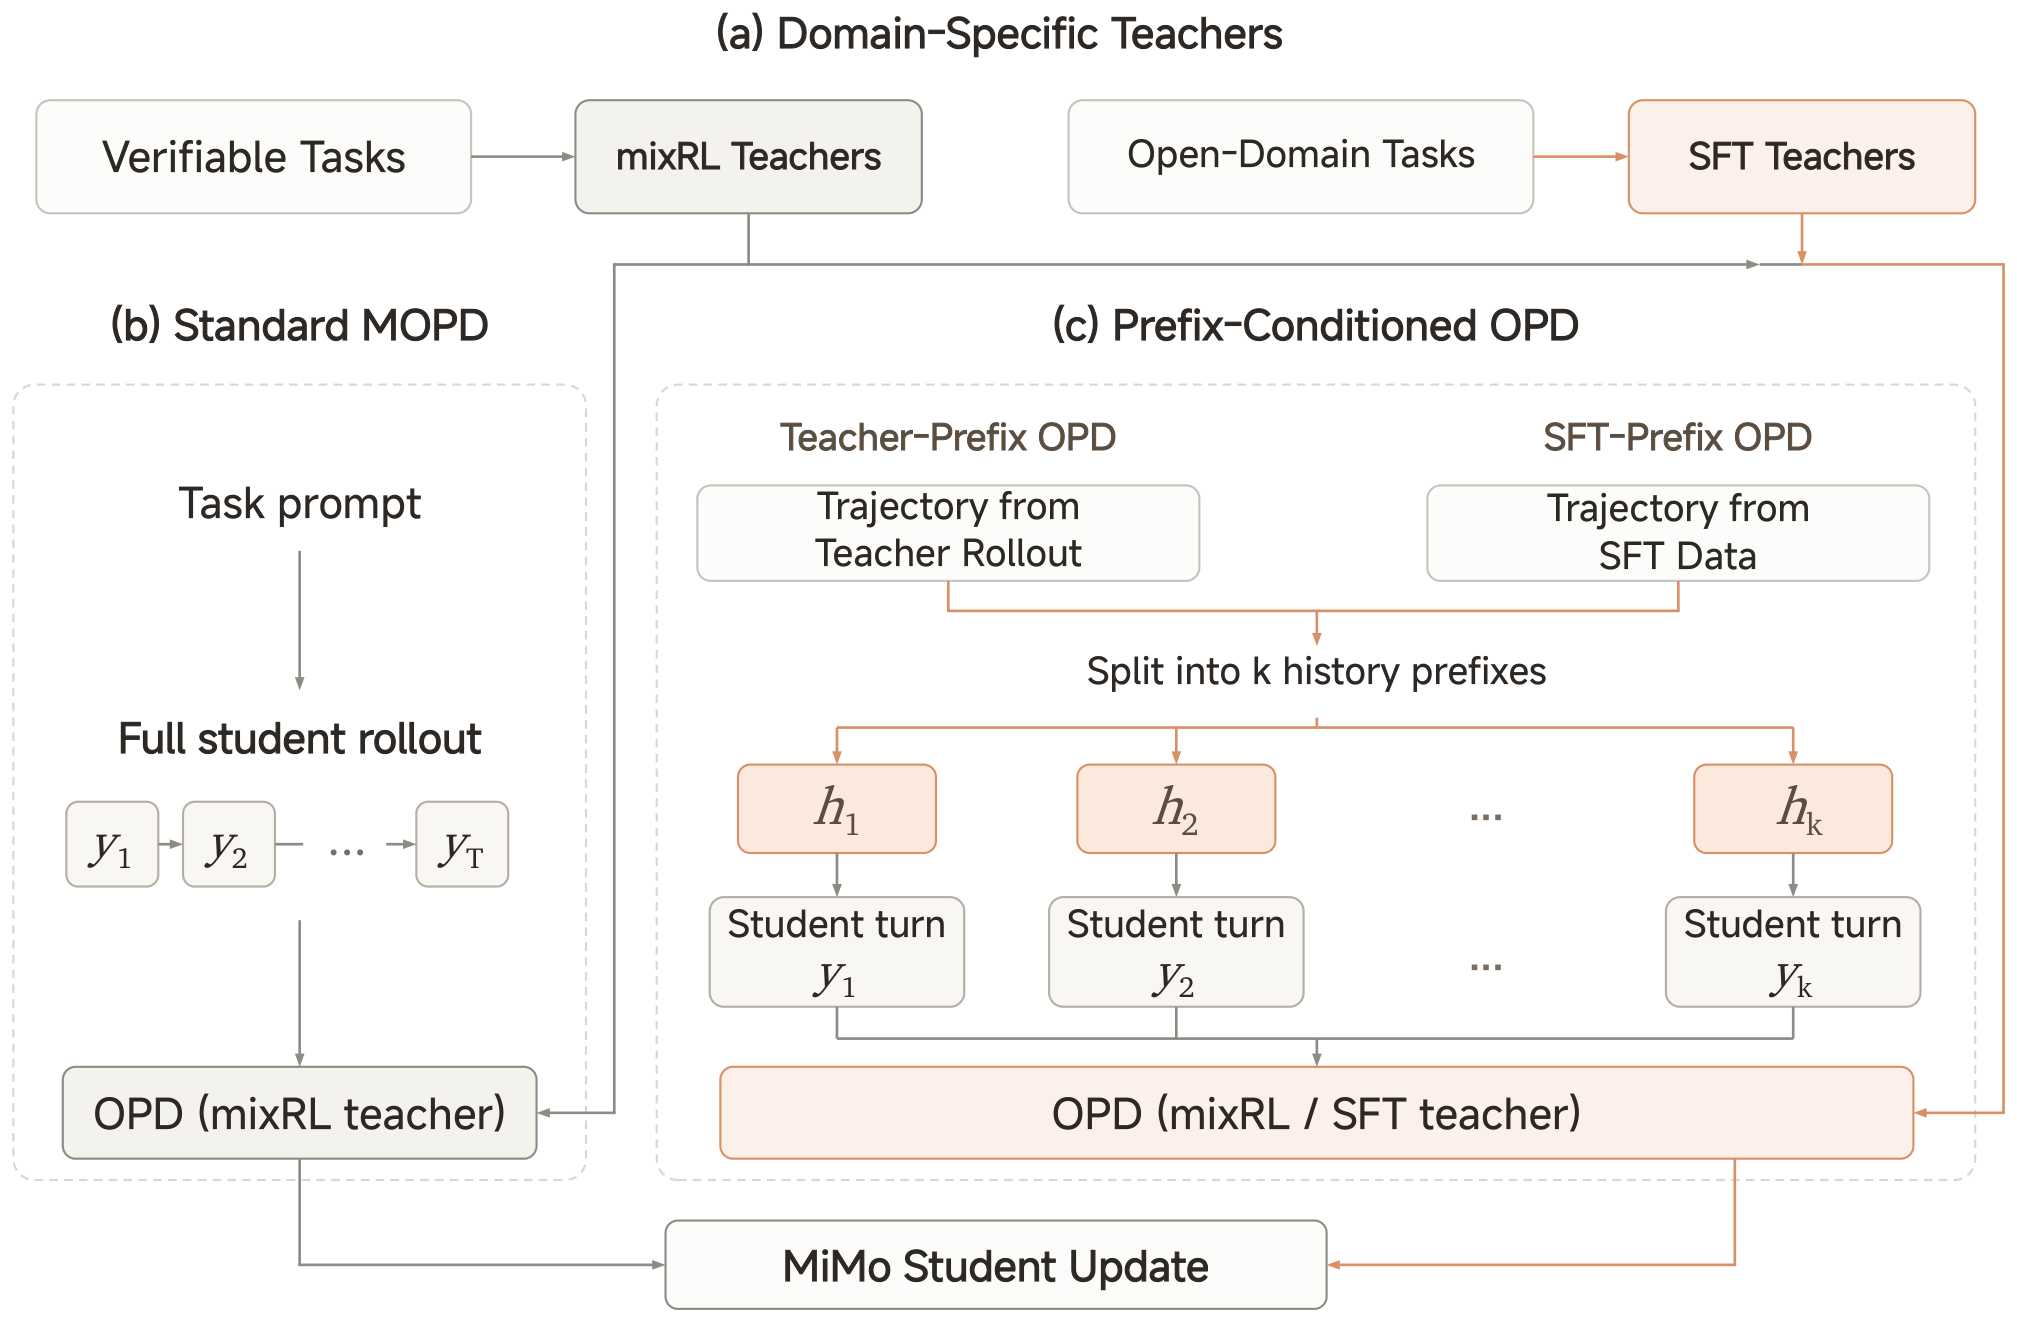
\includegraphics[width=\linewidth]{images_hi/fig13.png}
\caption{MiMo MOPD2 概览。(a) 领域专用教师在可验证任务上用 MixRL 训练，或在开放域任务上用合成演示做 SFT。(b) 标准 MOPD 用 RL 教师监督学生的完整 rollout。(c) 前缀条件 OPD 复用教师 rollout（Teacher-Prefix OPD）或 SFT 数据（SFT-Prefix OPD）中的轨迹。一条含 $k$ 个助手轮次决策点的源轨迹可得到 $k$ 个完整历史前缀 \(h _ { i } ,\)，每个前缀都可初始化一个单独由学生生成的轮次 \(y _ { i }\)，供相应领域教师做 token 级蒸馏。SFT 数据提供的是前缀上下文，而非固定的续写目标。}
\label{fig:13}
\end{figure}

前缀来自教师 rollout（Teacher-Prefix OPD）或 SFT 数据（SFT-Prefix OPD）。
一条含 $k$ 个助手轮次的轨迹提供 $k$ 个完整历史前缀，每个前缀在对应轮次之前
结束。学生从每个前缀采样一个新轮次，不重新生成此前的交互。预先指定的教师
以相同历史和学生的前序 token 为条件提供 token 级监督。

对于难以设计可靠 RL 奖励的开放域任务，我们用高质量合成演示训练 SFT 教师。
这类训练对长时程任务中学生反复偏离后所到达的历史覆盖可能有限
（Xu et al., 2025）。因此 SFT-Prefix OPD 让每次 rollout 都从固定的演示前缀
开始，限制采样轮次之前的偏离。演示提供上下文，学生则生成自己的续写，而不是
模仿固定回答。

MOPD2 进一步把 RL 训练模型的能力扩展到难以进行可靠训练时验证的领域，包括
环境复杂或校验器难以设计的领域，例如长时程游戏开发、科学研究和具身智能。
MiMo-V2.6 的最终评测结果见表 3。MiMo-V2.6 系列相对 MiMo-V2.5 有大幅提升，
在多个领域达到与前沿模型相当的表现。




{\footnotesize\setlength{\tabcolsep}{3pt}
\begin{longtable}[]{@{}|L{13em}|C{7em}|C{7em}|C{7em}|C{7em}|C{7em}|C{7em}|@{}}
\caption{MiMo-V2.6 与上一代模型及前沿模型在智能体基准上的对比。}\label{tab:3}\\
\toprule\noalign{}
\endfirsthead
\multicolumn{7}{r}{（续表）}\\
\toprule\noalign{}
\endhead
\bottomrule\noalign{}
\endlastfoot
\hline
基准 & MiMo-V2.6 Pro & MiMo-V2.6 Flash & MiMo-V2.5 Pro & Claude
Opus 5 & GPT-5.6 Sol & Claude Fable 5 \\
\hline
\multicolumn{7}{@{}l@{}}{%
代码智能体} \\
\hline
DeepSWE v1.1 & 71.9 & 67.9 & 19.0 & 74.0 & 73.0 & 70.0 \\
\hline
ProgramBench & 26.5 & 26.0 & 12.5 & 37.0 & 25.0 & 33.0 \\
\hline
MiMo Code Bench & 63.2 & 61.2 & 40.4 & 68.6 & 59.3 & - \\
\hline
\multicolumn{7}{@{}l@{}}{%
通用智能体} \\
\hline
AutomationBench v1.0.6 & 53.1 & 52.3 & 16.0 & 50.3 & 45.8 & 46.2 \\
\hline
Toolathlon-Verified & 76.9 & 73.6 & 49.1 & 80.6 & 74.9 & 77.9 \\
\hline
GDPval-AA 2.1 & 1673 & - & 1107 & 1708 & 1588 & 1595 \\
\hline
Agents\textquotesingle{} Last Exam & 31.6 & 27.6 & 13.2 & 31.6 & 30.8 &
25.7 \\
\hline
Terminal Bench 4.0 & 34.9 & 28.8 & 1.5 & 49.0 & 39.9 & 42.4 \\
\hline
Terminal Bench 2.1 & 89.9 & 87.6 & 65.2 & 89.1 & 88.8 & 84.3 \\
\hline
OSWorld-Verified & 82.0 & 80.8 & - & 83.4 & 83.0 & 86.0 \\
\hline
JobBench & 62.0 & 61.2 & 25.0 & 65.7 & 45.4 & 57.4 \\
\hline
\multicolumn{7}{@{}l@{}}{%
网络安全} \\
\hline
CyberGym & 94.0 & 95.1 & 40.0 & - & - & - \\
\hline
MiMo Cyber Bench & 80.2 & 77.2 & 0.0 & - & - & - \\
\hline
ExploitGym & 17.8 & 6.0 & 0.2 & 22.1 & 30.3 & 28.4 \\
\hline
ExploitBench & 47.9 & 25.3 & 16.6 & 70.0 & 78.5 & 78.0 \\
\hline
SEC Bench Pro & 66.3 & 47.5 & 17.7 & - & 79.1 & - \\
\hline
\multicolumn{7}{@{}l@{}}{%
视觉智能体} \\
\hline
MiMo Visual Coding & 72.3 & 71.5 & - & 70.0 & 73.4 & 69.1 \\
\hline
\end{longtable}
}

\section{RL 与 OPD 基础设施}\label{rl-and-opd-infrastructure}

MiMo-V2.6 系列将 RL 与 OPD 训练扩展到由智能体 rollout 构成的大规模混合任务批。为支持灵活的智能体 rollout 场景，我们定义了执行模型与轨迹数据结构，并用惩罚模块（Penalty Module）细化学习信号（§6.1）。在大批大小下，我们实现 Harness Pool 来承载多个脚手架并维持高 rollout 并发，实现 Payload Porter 来缓冲数万条携带路由与多模态数据的重型轨迹（§6.2）。我们实现 Sample Mixer，它与动态采样器和部分 rollout 协同，稳定地产出符合指定训练分布的训练批（§6.3）。为稳定高效的 RL 训练，我们在训练引擎与推理引擎之间对齐 MoE 路由与 top-p 采样候选集，同时针对 RL 负载优化这两个引擎（§6.4）。

\subsection{细粒度学习信号的智能体 RL}\label{agentic-rl-with-fine-grained-learning-signals}

智能体 rollout 跨越多轮与多个对话上下文，而结果奖励只提供粗粒度监督。因此我们采用以智能体为中心的执行模型，并把轨迹数据组织为层次结构。在该层次结构内，可配置的惩罚模块施加损失掩码与优势塑形。它针对模型自身的局部错误，并把基础设施故障排除在训练信号之外。



Agent Loop 我们把 rollout 从以推理为中心的设计转向以智能体为中心的设计：每条序列作为一个 Agent Loop 运行，它拥有环境生命周期、管理自己产生的对话，并按需调用推理引擎。生命周期涵盖建立、交互、奖励评估（例如运行测试用例）与清理。交互期间，loop 暴露一个请求端点，外部智能体通过调用它来驱动 rollout。每段对话同时以字符串前缀和 token 序列两种形式保存。前缀匹配定位到来请求所扩展的那段对话，只对新后缀做分词并送入推理引擎，使其接口保持纯粹的 token 进、token 出。

轨迹层次结构 子智能体、上下文压缩与多种智能体角色会在一次 rollout 内产生并发的对话分支。我们把轨迹数据组织为四级层次：Sample $\to$ Sequence $\to$ Context $\to$ Segment。Sample 是由 Sample Mixer 派发的一条提示（§6.3）。在 GRPO（Shao et al., 2024）这类组内算法中，一个 Sample 派生出一组 Sequence，该组作为整体被接受或拒绝。一个 Sequence 是一次 Agent Loop 执行，可包含多个并发 Context。一个 Context 是一条对话分支，持有一个 Segment 列表；它是前缀匹配、KV 缓存复用与训练数据导出的单位。一个 Segment 是单轮——一条系统或用户消息、一次模型生成，或一个工具结果——只有模型生成的轮次参与损失。

惩罚模块 组内算法把结果奖励均匀分摊到一条序列中所有模型生成的 token 上。在上述层次结构中，功劳很少是均匀的：有些轮次偏离路径或退化，有些失败与模型无关。为把功劳归于应得之处，我们把检测与其对训练的影响分开。Rule 通过手工逻辑或基于模型的裁判来评判一个 segment、context 或 sequence。例如，规则可以捕捉不可归因于模型的基础设施故障、乱码 token 模式、对不可用工具的调用以及重复。Strategy 把一个动作绑定到层次结构的某一层：mask 把命中的内容排除出损失，优势塑形对命中 token 上的优势进行设置、缩放或减去，monitor 只记录指标。复合的 early stop 策略在其规则触发时立即终止 rollout，把结果奖励置零，对触发轮次与更早的轮次施加不同的动作，并掩蔽同级 context。惩罚沿层次结构逐级升级：没有存活模型轮次的 context 被丢弃，没有存活 context 的 sequence 获得零优势，没有存活 sequence 的 sample 被拒绝。训练中实际施加的具体惩罚见 §4.3.3。

\subsection{Harness Pool 与 Payload Porter：多脚手架的大批大小 RL}\label{harness-pool-and-payload-porter-large-batch-rl-with-multiple-harnesses}

把 RL 训练扩展到大批会提高 rollout 并发度，也提高轨迹数据的内存与通信开销。混合任务批又增加了异质性的一个维度：单个批混合多个脚手架，每个训练样本组绑定到一个脚手架。在执行侧，Harness Pool 把并发的脚手架实例与 Agent Loop 托管在常驻的多租户 actor 池中，脚手架代码库、智能体行为与环境设置各自独立配置。在数据侧，Payload Porter 让 driver 仅凭轻量元数据完成调度。重型 payload 一次性写入分布式存储，并在被消费处打包。多模态 payload 按同样方式拆分为元数据与像素，并采用增量传输与负载均衡编码。




\begin{figure}[htbp]
\centering
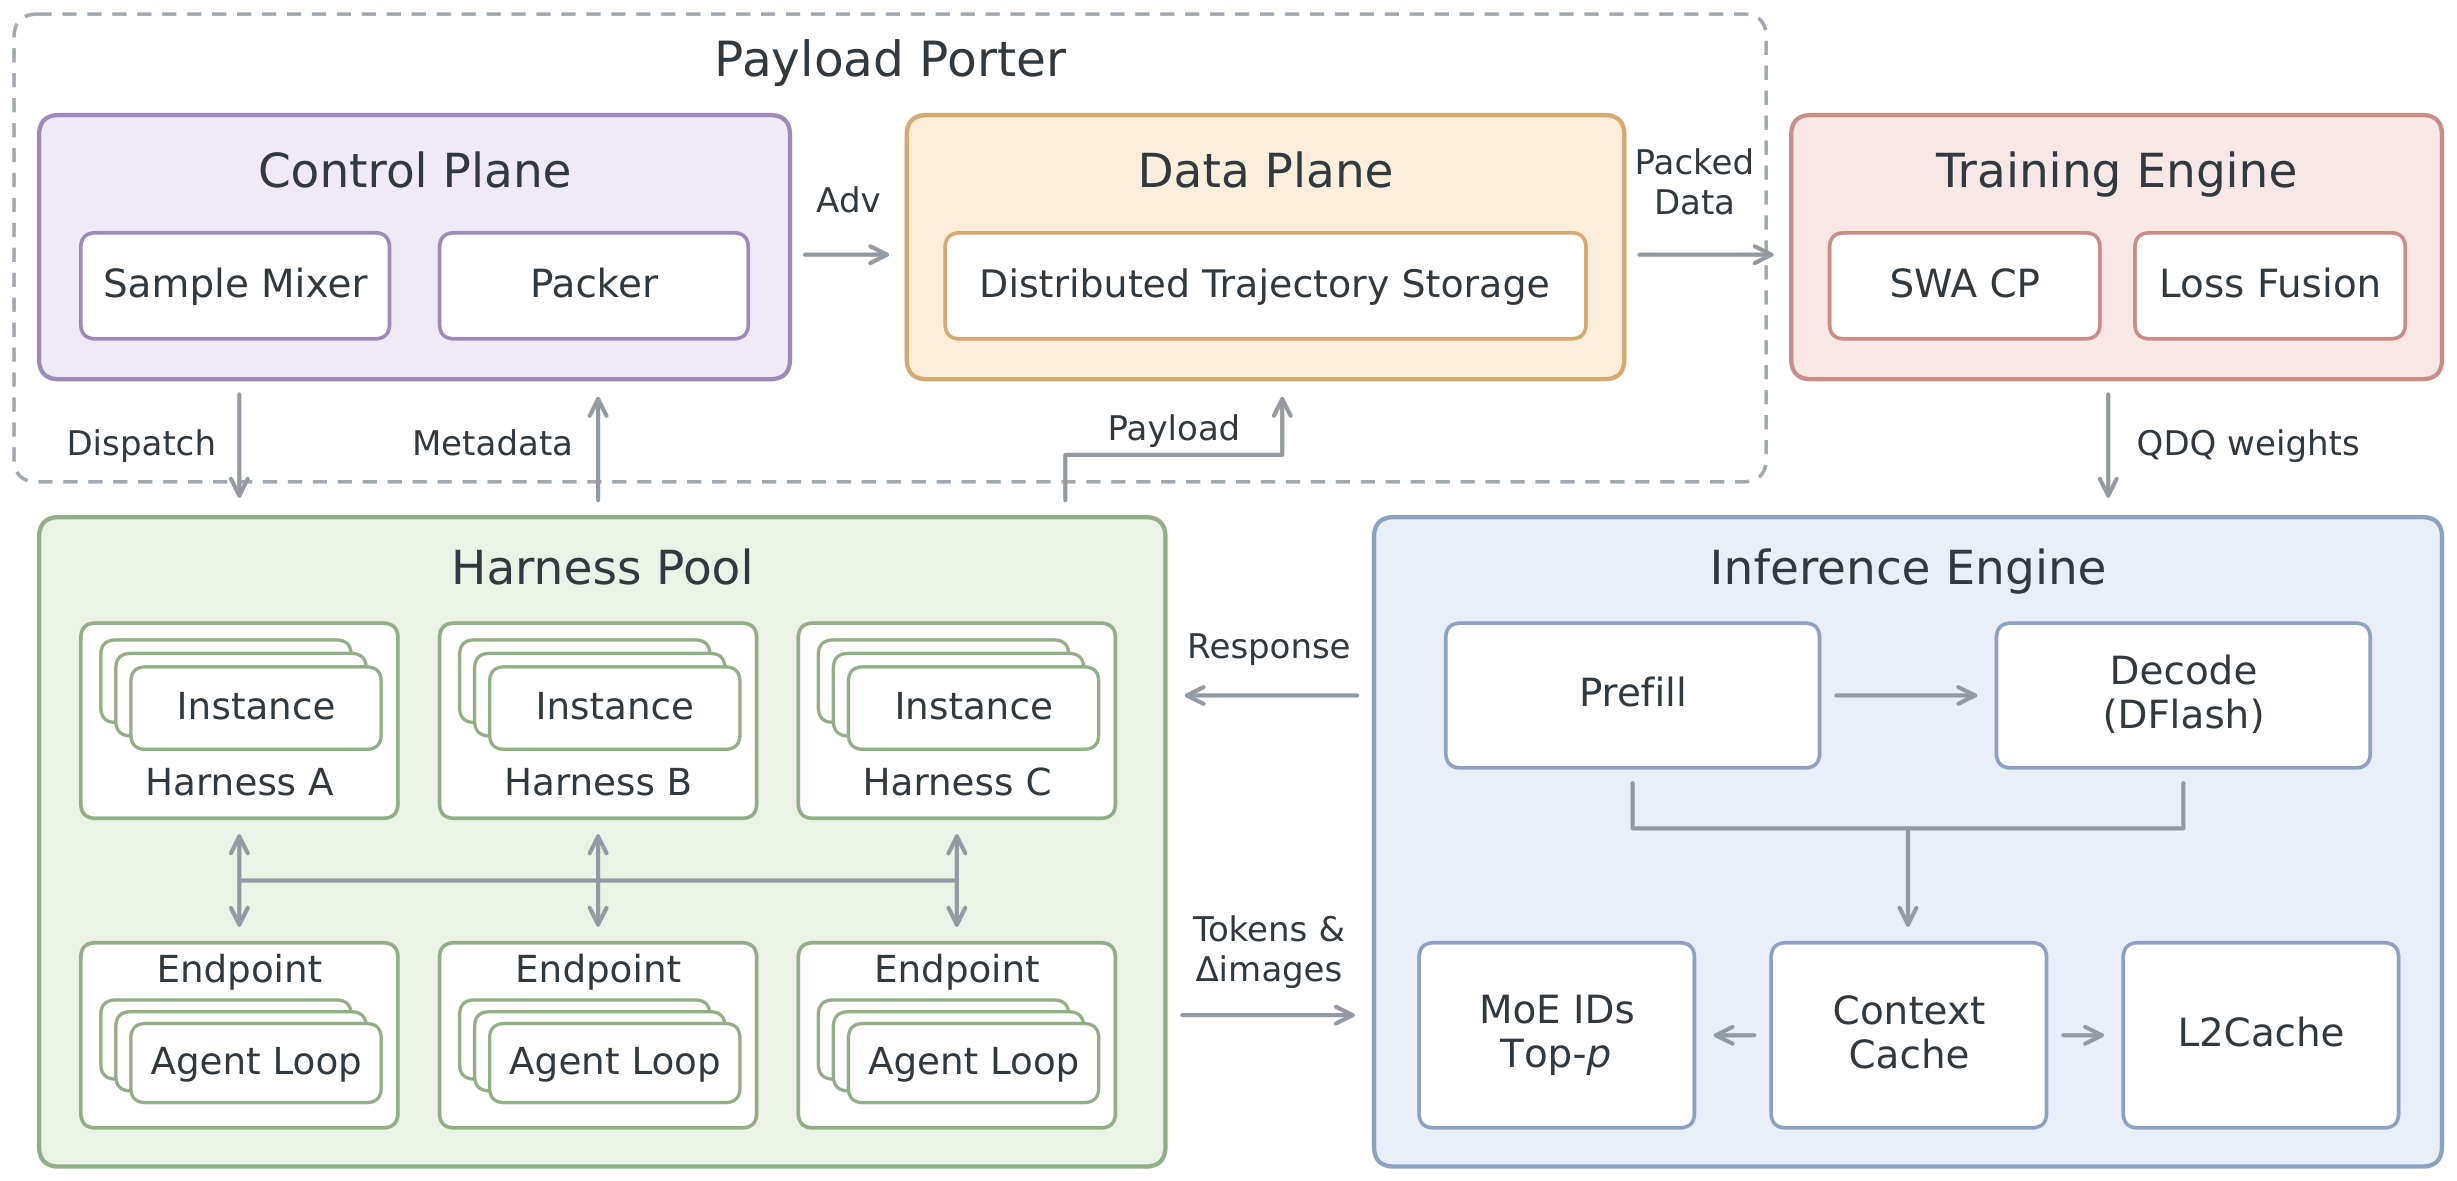
\includegraphics[width=\linewidth]{images_hi/fig14.png}
\caption{RL 基础设施的总体架构。}
\label{fig:14}
\end{figure}

多租户 rollout 执行 我们用 Ray actor（Moritz et al., 2018）在集群上执行智能体脚手架与 Agent Loop。若为每个脚手架实例和 Agent Loop 都分配一个专用 Ray actor，会在 Ray 的全局控制存储（GCS）节点上为每个 actor 占用一个文件描述符，而大批会耗尽 GCS 节点的文件描述符。我们改为运行固定大小的常驻 host actor 池，每个 host 承载许多并发租户——模型侧的 Agent Loop 与环境侧的脚手架实例。每个租户保持自己的轨迹状态，分配按在途实例数做均衡。一个 host 是一个单一进程，其租户共享一个事件循环。模型侧的租户还共享一个请求端点、一个推理代理和一个分词器；环境侧的租户共享一个已导入的脚手架代码库。共享事件循环会让一个阻塞调用拖住所有租户，因此阻塞型工作——环境操作与分词——放在后台线程上运行。这样把进程与服务开销摊销到并发 rollout 上，从而支持更大的并发批，而 actor 数量不会成比例增加。

异构智能体脚手架 我们分别配置脚手架代码库、智能体行为与环境设置，以在单次训练运行中容纳多样的任务。不同数据源可以使用不同的代码库，而智能体配置在同一数据源内随提示不同而变化。每个训练样本组使用统一配置，以便做组内相对优势估计。一个进程只能导入一个脚手架代码库，因此不同代码库运行在各自独立的池中。这些池从固定的 host actor 预算中获得可配置的份额——预算在启动时设定一次，与每步调度的训练数据配比无关。脚手架多样性与 rollout 并发度因此可以在同一个执行框架内扩展。

数据面与控制面分离 扩展后的批必须一次缓冲数万条序列，且每条都很重：除 token id 与对数概率外，还携带 MoE 路由数据、top-p 采样索引与多模态数据。payload 体量随序列数量与长度一同增长，而把所有 payload 汇聚到单个 driver 节点会使批大小受限于该节点的内存。因此我们把数据面与控制面分离，在 rollout 结束时对每条序列做切分：其 payload 一次性写入分布式键值存储（例如 Ray object store 或 TransferQueue（Han et al., 2025）），而 driver 仅凭轻量元数据完成全部调度——标量奖励、各 context 的长度，以及寻址每个 payload 的键。在组结束时，只从存储读取所需字段：accept-time 钩子需要的少数几列。组内评分器在配置后会与 Agent Loop 完全异步地运行——其延迟被隐藏，结果可以滞后——并在返回时改写组奖励。采样器随后仅凭元数据按通过率接受或拒绝该组，钩子则施加长度惩罚、计算组内相对优势并施加优势塑形。逐 token 优势被写回存储；优势全为零的组默认被丢弃。在 OPD 下，奖励评估被教师打分取代：每条轨迹被送往教师服务器，其分数被异步收集到同一个分布式存储中。在批产出时——即每个数据源都贡献了其在批中的份额之后——产出钩子把被接受的序列打包成微批并分配到各个 rank，不触碰任何张量。打包时，每个训练张量并行（TP）组由一个 packer 服务该组内的所有 rank。它从存储中未填充的行里，只取自己的上下文并行（CP）窗口覆盖到的行，并只切出该窗口。结果作为单个只读的内存副本在 TP 组内共享。这避免了 driver 上的全批聚合以及打包期间的稠密填充中间量。



多模态数据 多模态 payload 遵循同样的元数据/payload 拆分，但需要额外小心：随着智能体在多轮中反复截图和读取图像，单条轨迹可能累积数 GB 的此类数据——存储代价高，且随着历史增长重传代价也高。因此在 rollout 期间，Agent Loop 只发送请求之间的多模态增量（§6.4）。训练时，每个图像条目都必须经过视觉编码器。由于编码器在张量并行组内是复制的，而 LLM 主干是分片的，编码先以数据并行方式运行——图像条目在各 rank 间均衡分配，与各序列 token 的落点无关。编码后，嵌入被重分配到持有对应 token 的 rank 上。payload 本身留在分布式键值存储中：负载均衡规划只读取条目元数据，像素只在编码器计算时取用。这在容纳不均衡的多模态负载的同时，限制了冗余的 payload 搬运。

\subsection{样本混合器：稳定的异步混合任务 RL}\label{sample-mixer-stable-asynchronous-mixed-task-rl}

自 MiMo-V2-Flash（Core Team et al., 2026）起，我们一直维护一个 Data
Scheduler，它面向跨数据源的指定训练分布，并配合动态采样器（Yu et al., 2025）与部分
rollout（Kimi Team, 2025）。混合任务 RL 必须在 rollout 时长与过滤率大幅波动的情况下仍保持该分布，
使每个数据源都能得到有效训练。在 25 个已画像的数据源上，平均生成 token 数与活跃 rollout 时长分别相差 90$\times$ 和 66$\times$（图 15），
这要求调度能够适应各数据源的工作负载。为应对这些挑战，我们实现了 Sample Mixer，
用四种机制填充指定训练分布：自适应 rollout 并发设定各数据源的预算，
自适应 rollout 调度在预算内选择数据源，预测式 rollout 派发将新的 rollout 放置到各 rank，样本
回放则覆盖启动与恢复阶段。

自适应 rollout 并发 较慢的数据源需要更多并发
rollout，才能维持相同的训练贡献。对数据源 $i$，设
\(B _ { i }\) 表示每个训练步目标保留的样本组数，\(r _ { i }\) 为估计的组接受率，
\(t _ { i }\) 为估计的活跃 rollout 时长，包含模型
生成与环境交互，但不含训练步之间的暂停。期望生成需求为 $m \_ \{ i \} = \{ B
\_ \{ i \} \} / \{ r \_ \{ i \} \} ; $；在固定训练吞吐下，
所需并发随 \(t _ { i } m _ { i }\) 增长。我们为每个数据源分配
\(( 1 + p _ { i } ) m _ { i }\)
组的调度预算，其中过采样比 \(p _ { i }\) 满足



\begin{figure}[htbp]
\centering
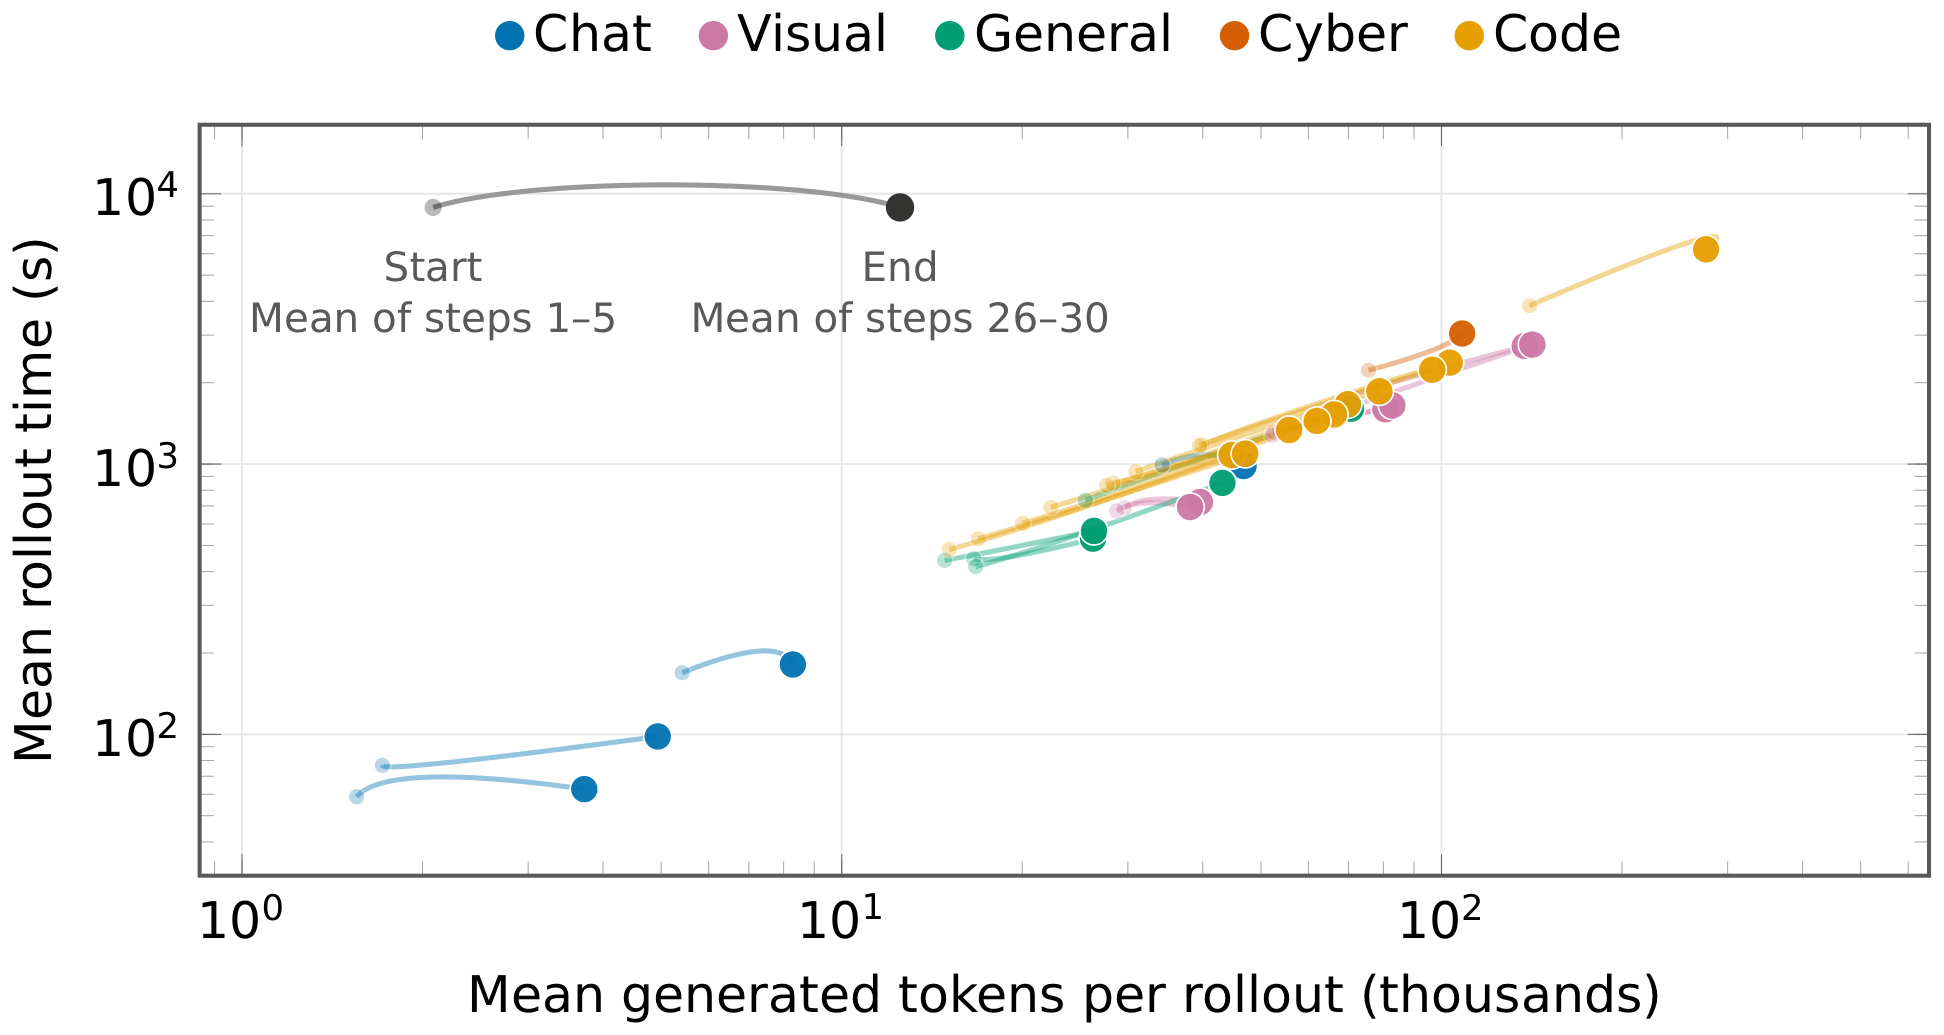
\includegraphics[width=\linewidth]{images_hi/fig15.png}
\caption{25 个数据源上的 rollout 异质性。每条线连接一个数据源的 Start 点（浅色）与其 End 点（实线）；每个点画出该数据源在已完成 rollout 上的平均生成 token 数与平均 rollout 时间（token 在上下文过滤前跨对话上下文求和）。两个坐标轴均为对数尺度。}
\label{fig:15}
\end{figure}


\[
p _ { i } = \mathrm { c l i p } ( c t _ { i } - 1 , p _ { \mathrm { m i n } } , p _ { \mathrm { m a x } } ) , \qquad \frac { \sum _ { i } m _ { i } p _ { i } } { \sum _ { i } m _ { i } } = \bar { p } .\tag{6}
\]

共享因子 $c$ 将 \(p _ { i }\) 的需求加权均值保持在
全局过采样比 \({ \bar { p } } ,\) 处，并受各数据源上界约束。我们随工作负载变化，依据近期计时与接受
统计重新计算该分配。在稳态下，并发
需求随数据源的 rollout 时长与目标增长，随其接受率下降。

自适应 rollout 调度 在这些预算内，调度在长期生成需求
与当前训练批的推进之间取得平衡。若当前批已从数据源 $i$
接受 \(A _ { i }\) 组，则其调度权重为

\[
w _ { i } = \alpha \frac { B _ { i } } { r _ { i } } + ( 1 - \alpha ) \frac { ( B _ { i } - A _ { i } ) ^ { + } } { r _ { i } } ,\tag{7}
\]

其中 \(( x ) ^ { + } = \operatorname* { m a x } ( x , 0 )\)，且
\(\alpha \in [ 0 , 1 ]\)。目标项维持生成需求；
亏空项优先考虑仍有亏空的数据源。这些
权重驱动平滑加权轮询；稳态启动将
\(\alpha = 0 . 5\) 与按 \(t _ { i } m _ { i }\) 比例分配的初始并发结合使用。图 16 的轨迹驱动仿真
在固定并发上限、数据源预算不构成约束的条件下比较了这些策略：在该工作负载下，亏空校正调度 \(( \alpha = 0 . 5 )\)
相比基于亏空的调度
\(\left( \alpha = 0 \right)\) 提升了占用稳定性，相比基于目标的
调度 \(( \alpha = 1 )\) 改善了收集均衡性。仿真时长按图 15 中各数据源
在 End 处的平均 rollout 时间校准。

预测式 rollout 派发 我们联合估计 KV 需求与期望
推理并发，以指导新 rollout 在各 rank 上的准入与放置。按数据源先验估计一个 rollout 的总
序列长度（输入与生成 token），跨上下文求和；
这些先验由已完成的 rollout 更新，并用于估计 KV
需求。仅当一个 rollout 估计 KV 需求的安全余量倍数
能放入目标 rank 剩余的 GPU KV
容量时，我们才准入该 rollout。分层缓存（§6.4）横跨 HBM 与锁页主机内存池：
两层共同保留已准入 rollout 的状态。rollout 时间中用于环境执行的
估计占比将 rollout 并发转换为期望推理并发。我们
用 CUDA graph 捕获所用的最大运行请求数来约束该期望值，从而限制会延长 rollout 生命周期并
增加陈旧度的排队延迟。为在两种约束下最大化吞吐，一个
贪心启发式选择剩余容量最大的可行 rank——即可用并发槽位与剩余 KV
容量（均以序列为单位表示）中的较小者——并在每次放置后更新这两个量。




\begin{figure}[htbp]
\centering
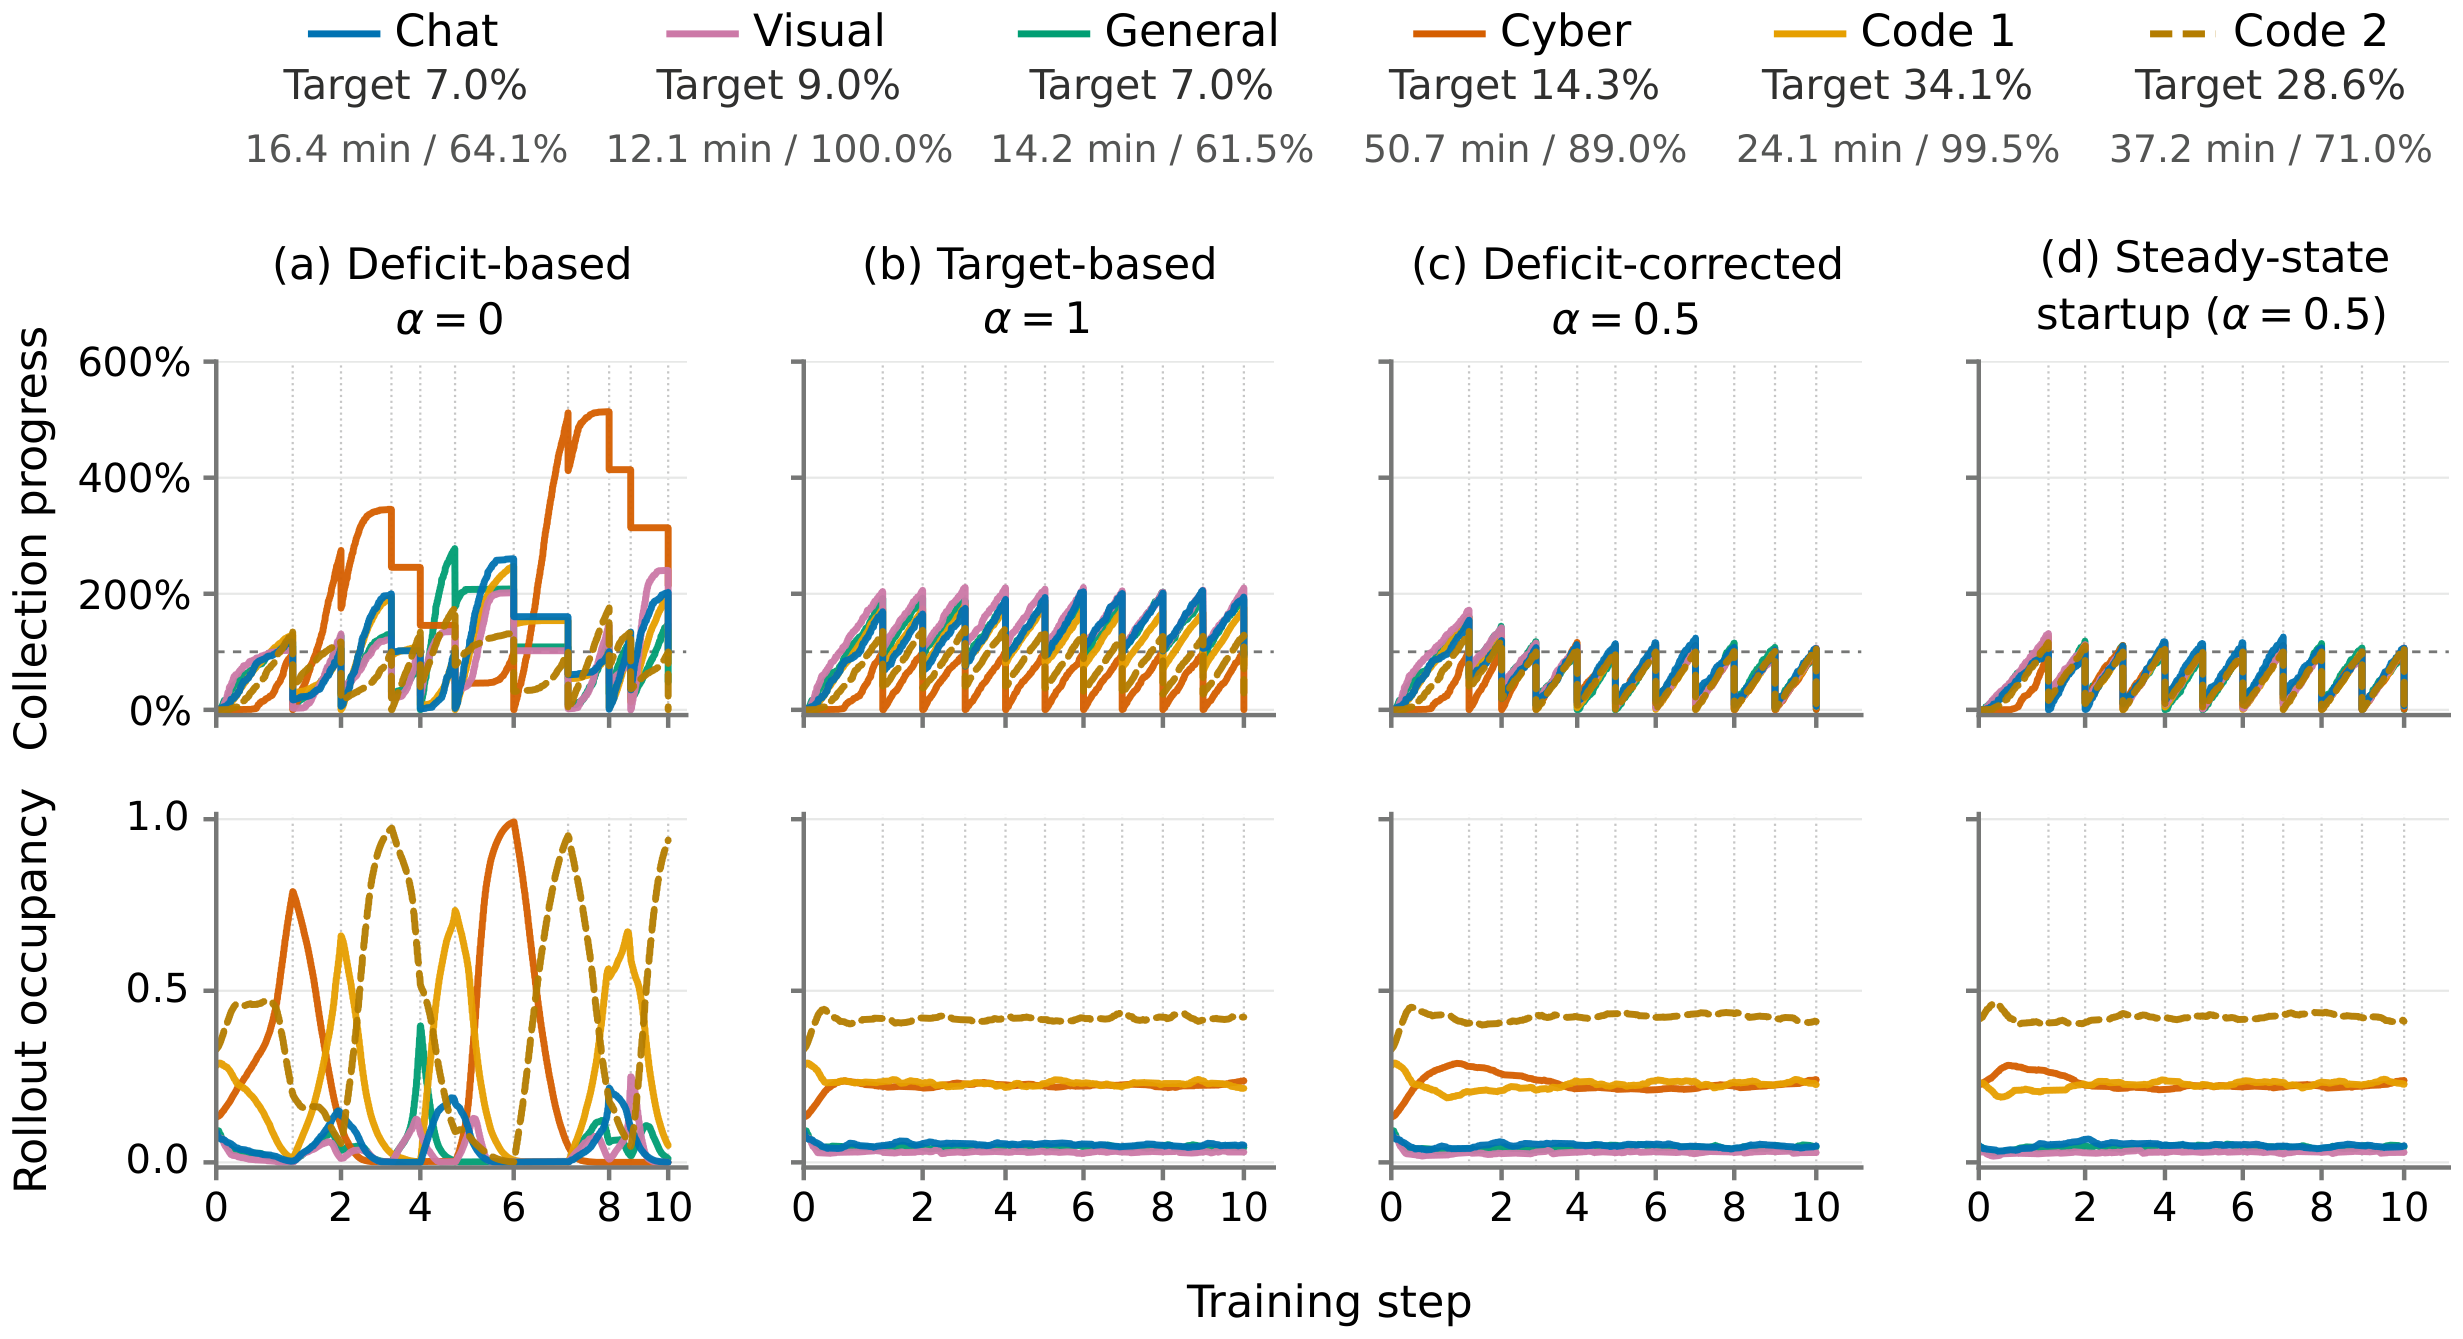
\includegraphics[width=\linewidth]{images_hi/fig16.png}
\caption{六个数据源的轨迹驱动调度仿真。图例：平均时长 / 组接受率。上：收集进度（已接受组数 / 每步名义目标，盈余结转）。下：rollout 占用（已占用序列槽位的份额）。步间距反映经过的时间。虚线标出步边界。训练时间、信用分配延迟、陈旧过期与回放不计入。}
\label{fig:16}
\end{figure}


样本回放 我们使用样本回放来加速从
慢数据源的初始收集。在画像中，启动阶段的样本收集耗时约为持续运行的
1.8$\times$。在慢数据源内部，
较短的 rollout 往往先完成，即使各数据源目标已达成，也会使初始批次
产生偏差。因此，我们在启动或检查点恢复后的第一个收集步中，
复用来自选定慢数据源的已完成 rollout
组，在当前过滤规则下补齐各数据源剩余的亏空。全新启动回放假定
所存 rollout 是在该运行起始策略下生成的；恢复回放则
复用恢复前生成、且仍在各数据源陈旧上限内的已完成 rollout。将回放限制在第一个
收集步，可减少对慢数据源的等待，同时保持
指定的训练分布。



\subsection{训练/推理一致性与优化}\label{traininginference-consistency-and-optimization}

我们扩展 MiMo-V2-Flash（Core Team et
al., 2026）的 RL 与 OPD 基础设施，仍以 SGLang（Zheng et al., 2024）和 Megatron-LM（Shoeybi
et al., 2019）分别作为推理引擎与训练引擎。在
MiMo-V2.6 中，我们在 rollout 期间使用 MXFP4 作为专家的数据类型。我们
在混合专家（MoE）路由与概率归一化上保持两个引擎
对齐。推理侧，
Context Cache 在跨轮次携带 KV 状态的同时携带路由记录、采样候选集与
视觉输入，并将空闲状态卸载到主机内存。一个在 RL rollout 日志上训练的
草稿模型通过推测解码进一步
加速生成。训练侧，我们降低长序列的内存与通信开销。

训练--推理一致性 为支撑 MiMo-V2.6 系列，我们在每次参数
更新后对专家应用量化--反量化（QDQ）。该量化遵循 rollout 期间
所用 MXFP4 Humming GEMM 内核（vLLM Project, 2026）的数值约束，因此
两个引擎看到完全相同的专家权重。即使参数相同，引擎间的数值差异也可能
改变离散的专家选择；Rollout Routing Replay（R3）（Ma et al., 2025）记录
rollout 期间使用的专家索引，并在训练期间重放它们，
复现所捕获的执行路径。Top-k 与 top-p 采样在受限候选集而非全
词表上重新归一化；我们在 rollout 期间记录每个 token 的候选集（Liu et
al., 2025a; The Microsoft AI Team, 2026），并在其中重新归一化训练的
对数概率，以匹配采样器的归一化。对于
top-p 采样，只有 GPU--CPU 传输是稠密的：我们传输一个固定形状、全词表宽度的位图。
固定形状避免了 GPU--CPU
同步；全宽度则绝不会截断即使跨越
整个词表的候选集。后续所有阶段都是稀疏的：在典型的 top-p
0.97 下，候选集平均不到五个 token。R3 与 top-p
候选集重放的开销都可以忽略，因为负载保持
紧凑，并且不落在关键路径上。

上下文缓存 沿用 MiMo-V2-Flash
（Core Team et al., 2026）的请求级 KVCache，每个对话上下文都有一个持久键：
在同一个策略版本内，后续轮次命中已缓存的 KV——包括
生成的 token——只对新后缀做 prefill。上下文缓存是一个
刻意的有状态选择：缓存状态的生命周期长于每一轮。
因此，专家索引与候选集不会在
中间轮次返回，只在 rollout 最终被收集时返回，
避免了碎片化的逐轮通信与处理。历史
多模态输入既不需要重新哈希，也不需要重新发送：其视觉
token 已经位于缓存的 KV 中。只有新引入的图像
跨进程边界；完整视觉输入仅在
策略更新或缓存未命中后发送。多轮环境交互将
一条轨迹的墙上时钟划分为 GPU 时间（生成）与工具时间
（等待环境）；缓存的层次化扩展
将这种时间划分在空间上体现出来——状态在
GPU 时间驻留于 HBM，在工具时间驻留于锁页主机内存池。卸载与
恢复在旁路 CUDA 流而非计算流上运行，
绝不会阻塞生成。由此，HBM 尽可能用于运行中的请求：
解码批越大，算术
强度与算力利用率越高。

草稿模型加速 RL rollout 默认使用 block-6 DFlash 进行推测
解码，取代从 SFT 继承的多 token 预测（MTP-3）
配置。DFlash 最初在 SFT 策略上训练，
随后在重采样以匹配
RL 训练分布的早期 RL rollout 日志上微调。在该默认配置下，平均
接受长度比 MTP 配置高 31.3\%。在
较大的 RL 批大小下，我们依据端到端
吞吐而非仅凭接受率来选择草稿块大小。更小的草稿块
减少验证工作量：在混合任务 RL 评测中，block-6 相比 block-8 将
全局平均吞吐提升约 6\%，而平均接受长度变化
很小。低精度草稿计算（FP8）
也被用于降低起草开销。在我们的长上下文
工作负载上，经 RL 适配的 FP8 DFlash 相比基线取得约 10.3\% 更高的
单节点吞吐。



训练优化 我们以 1M token 的上下文长度训练 RL。
MiMo-V2.6 将 128-token 滑动窗口层与全
注意力交替堆叠。在上下文并行下，滑动窗口层只交换
其查询能触及的 KV——至多一个窗口大小的
片段——因此每层通信量由窗口而非
序列长度决定。长序列还会抬高内存占用，
MoE 专家不均衡则进一步推高峰值内存。优化器状态保存在
CPU 内存中，仅在参数更新时拷回。所有损失
计算融合进一个内核：策略梯度损失（带或不带 top-p 重新归一化）
与 OPD 损失，可选地连同熵、标签 logit、top-p 概率质量等指标。该融合节省内存
并缩短步时间。

\section{面向智能体 RL 的开放基础}\label{open-foundations-for-agentic-rl}

MiMo-V2.6 系列展示了强化学习在显著提升智能体能力方面的潜力。在此基础上继续推进，需要能力足够强的模型，以及能将有意义任务与可靠校验器配对的高质量 RL 环境。把这些资源连同可复现的基线一并公开，有助于开源社区持续开展研究与创新。因此我们开源了 MiMo-V2.6-Distill-Qwen-9B\footnote{\url{https://huggingface.co/XiaomiMiMo/MiMo-V2.6-Distill-Qwen-9B}}，一个从 MiMo 蒸馏得到的小模型，作为后续 RL 训练的共享起点。除模型之外，我们还发布了高质量的 RL 环境以及一套端到端的开源 RL 框架。本节中，我们使用这些已发布的资源建立各领域的 GRPO 基线。我们还在编码任务上做了一项独立的多脚手架训练实验作为案例研究，沿用 MiMo-V2.6 所描述的方法。实验显示多个领域都取得了显著提升，说明这些资源对 RL 训练具有价值。

\subsection{从 MiMo-V2.6 蒸馏}\label{distillation-from-mimo-v2.6}

扩展 RL 算力、扩大环境与脚手架的覆盖面，会带来更多探索与学习的机会。在这些场景中，有效的探索依赖于协调动作并对环境反馈作出响应。因此，释放智能体 RL 的潜力，首先要有一个扎实的任务求解能力基础。

为给开源社区提供这样一个基础，我们通过将 MiMo 的智能体经验迁移到更小的模型中，开发了 MiMo-V2.6-Distill-Qwen-9B。该模型由 Qwen3.5-9B (Qwen Team, 2025) 在 MiMo 生成的数据上监督微调得到，数据覆盖编码、通用领域、视觉和网络安全任务。该数据混合共含 774 亿 token，其中 272 亿为参与 SFT 目标的 loss token。表 4 汇总了数据组成。

得到的 MiMo-V2.6-Distill-Qwen-9B checkpoint 在各项报告的评测上均优于 Qwen3.5-9B（表 6）。例如 SWE-bench Pro (Deng et al., 2025) 从 32.0 提升到 44.6，AutomationBench 从 5.0\% 提升到 30.3\%。我们认为这些增强后的任务求解能力是进一步通过 RL 改进的良好基础。因此我们把该 checkpoint 作为下文各领域 GRPO 实验与多脚手架编码实验的共同初始化。




{\footnotesize
\begin{longtable}[]{@{}|l|l|l|l|@{}}
\caption{加权 SFT 数据组成。token 数量以十亿计。数值四舍五入到一位小数；总计使用未舍入的汇总计数。}\label{tab:4}\\
\toprule\noalign{}
\endfirsthead
\multicolumn{4}{r}{（续表）}\\
\toprule\noalign{}
\endhead
\bottomrule\noalign{}
\endlastfoot
\hline
数据来源 & 总 token 数（B） & token 占比（\%） & Loss token 数（B） \\
\hline
代码 & 23.2 & 29.9 & 7.3 \\
\hline
网络安全 & 11.0 & 14.2 & 4.8 \\
\hline
通用 & 22.0 & 28.5 & 5.7 \\
\hline
视觉 & 21.2 & 27.4 & 9.4 \\
\hline
总计 & 77.4 & 100.0 & 27.2 \\
\hline
\end{longtable}
}



{\footnotesize
\begin{longtable}[]{@{}|l|l|l|l|@{}}
\caption{已发布 RL 环境概览，包括训练任务数量以及用于判定任务完成情况的校验器。任务数为近似值，基于各训练集中不同的任务标识符统计；k 表示一千。}\label{tab:5}\\
\toprule\noalign{}
\endfirsthead
\multicolumn{4}{r}{（续表）}\\
\toprule\noalign{}
\endhead
\bottomrule\noalign{}
\endlastfoot
\hline
领域 & 任务族 & 训练任务 & 校验器 \\
\hline
代码 & 软件工程 & 3k & 可执行测试 \\
\hline
网络安全 & 漏洞复现 & 1k & 规则检查 \\
\hline
通用 & 知识工作 & 1k & 基于评分细则的评判 \\
\hline
视觉 & 网页开发 & 2k & 视觉评分 \\
\hline
\end{longtable}
}

\subsection{开放环境下的 RL}\label{rl-with-open-environments}

环境概览 表 5 汇总了我们发布的 RL 环境，覆盖编码、网络安全、通用领域和视觉任务。四个训练集总共约含 7k 个任务，其中通用领域集聚焦知识工作。训练资源还包含约 1k 个音乐生成任务，用于支持下文报告的 GRPO 实验。

RL 实验 从同一个 MiMo-V2.6-Distill-Qwen-9B SFT checkpoint 出发，我们使用对应的已发布环境，分别针对编码、网络安全、通用领域和视觉任务进行 GRPO 训练。除公开基准外，我们还评测四个内部集合：面向软件工程的 MiMo Code Bench (mini)、面向漏洞复现的 MiMo Cyber Bench (mini)、面向知识工作的 MiMo General Bench (mini)，以及面向网站开发的 MiMo Visual Coding (mini)。这些评测集遵循与其对应训练集相同的任务分布。

表 6 显示，RL 在表中报告的 11 项评测上相对 SFT checkpoint 均有提升，覆盖四个任务领域。SWE-bench Verified (Jimenez et al., 2024) 从 61.1 升至 66.2，Terminal Bench 2.1 (Merrill et al., 2026) 从 37.1 提升到 52.8。OfficeQA Pro (Opsahl-Ong et al., 2026) 从 19.5 提升到 24.8，Toolathlon-Verified (HKUST NLP, 2026) 从 35.2 升至 38.0。MiMo Visual Coding (mini) 从 64.0 提升到 72.4，MiMo Cyber Bench (mini) 从 31.3 升至 47.0。除表 6 报告的任务外，我们还探索了艺术创作与设计等新兴任务，例如音乐创作。在我们的内部音乐基准上，分数从 SFT 后的 45.7 大幅提升到 RL 后的 52.5。




{\footnotesize
\begin{longtable}[]{@{}L{17em}llll@{}}
\caption{Qwen3.5-9B、SFT 后的 MiMo-V2.6-Distill-Qwen-9B，以及进一步 GRPO 训练（RL）后各领域 checkpoint 的评测结果。代码使用单脚手架 RL。每行中的最高可得分数以粗体标出。}\label{tab:6}\\
\toprule\noalign{}
\endfirsthead
\multicolumn{5}{r}{（续表）}\\
\toprule\noalign{}
\endhead
\bottomrule\noalign{}
\endlastfoot
\multirow{2}{*}{基准} & \multirow{2}{*}{指标} &
\multirow{2}{*}{Qwen3.5-9B} & \multicolumn{2}{l@{}}{%
MiMo-V2.6-Distill-Qwen-9B} \\
& & & SFT & RL \\
\multicolumn{5}{@{}l@{}}{%
代码} \\
SWE-bench Verified & avg@3 & 60.0 & 61.1 & 66.2 \\
SWE-bench Pro & avg@3 & 32.0 & 44.6 & 47.6 \\
MiMo Code Bench (mini) & avg@3 & 19.5 & 51.6 & 59.9 \\
\multicolumn{5}{@{}l@{}}{%
网络安全} \\
MiMo Cyber Bench (mini) & avg@3 & 5.7 & 31.3 & 47.0 \\
\multicolumn{5}{@{}l@{}}{%
通用} \\
AutomationBench v1.0.6 & avg@1 & 5.0 & 30.3 & 33.1 \\
Terminal Bench 2.1 & avg@1 & 27.0 & 37.1 & 52.8 \\
Toolathlon-Verified & avg@1 & 25.9 & 35.2 & 38.0 \\
OfficeQA Pro & avg@1 & 9.0 & 19.5 & 24.8 \\
JobBench & avg@1 & 2.6 & 18.3 & 25.2 \\
MiMo General Bench (mini) & avg@1 & 28.5 & 62.2 & 70.6 \\
\multicolumn{5}{@{}l@{}}{%
视觉} \\
MiMo Visual Coding (mini) & avg@1 & 61.7 & 64.0 & 72.4 \\
\end{longtable}
}

这些结果凸显了高质量训练数据与强 SFT 初始化对进一步 RL 改进的价值。

多脚手架训练 表 6 中的编码结果通过单脚手架 RL 得到。我们在另一项编码实验中进一步研究多脚手架训练，同样从 MiMo-V2.6-Distill-Qwen-9B SFT checkpoint 出发。沿用 MiMo-V2.6 描述的多脚手架训练方法，我们在四个 mini-harness 上联合优化模型，并在这些脚手架以及另外三个留出（held-out）脚手架上评测。表 7 在三个编码评测和七个智能体脚手架上比较了 Qwen3.5-9B 与多脚手架 RL 前后的 MiMo-V2.6-Distill-Qwen-9B。MiMo-V2.6-Distill-Qwen-9B 在全部 21 个数据集--脚手架组合上优于 Qwen3.5-9B，多脚手架 RL 又进一步提升了每一组合。在 MiMo Code Bench (mini) 上，相对 SFT 的额外增益在七个脚手架上介于 1.8 到 9.3 个百分点之间。

案例研究 为更直观地展示我们的 SFT 与 RL 方案如何逐步增强模型能力，我们给出一个网页开发方向的案例研究（该领域的视觉质量一目了然），在图 17 中比较 Qwen3.5-9B、MiMo-V2.6-Distill-Qwen-9B (SFT) 与 MiMo-V2.6-Distill-Qwen-9B (RL) 生成的网站。如左列所示，Qwen3.5-9B 生成的网站在视觉设计上较为朴素，布局简单，图片使用很少。值得注意的是，(c) 中的人力资源管理界面存在明显的布局问题。经过蒸馏后，MiMo-V2.6-Distill-Qwen-9B (SFT)（中列）生成的网站内容明显更丰富，配色更协调，图像素材的运用也更有效，例如 (b) 中埃塞俄比亚遗产页面的摄影元素。经过 RL 训练后（右列），模型更进一步，给出最精致的结果：排版考究、hero 区域视觉冲击力强（如 (b) 中的日落图像），页面布局也更完整、结构更清晰（如 (c) 中功能齐全的人力资源仪表盘，带有侧边导航、日历组件和详细的统计卡片）。这些逐步的定性改进与表 6 中观察到的定量轨迹（61.7 $\to$ 64.0 $\to$ 72.4）一致，共同说明先从 MiMo-V2.6 蒸馏再经 RL，能累积提升生成结果的美学质量与功能完整度。




{\footnotesize\setlength{\tabcolsep}{3pt}
\begin{longtable}[]{@{}L{14em}C{5em}C{5em}C{5em}C{5em}C{5em}C{5em}C{5em}C{5em}@{}}
\caption{各智能体脚手架上的编码表现。均值为七个脚手架分数的未加权平均，四舍五入到一位小数。每个数据集内各列的最佳结果以粗体标出。}\label{tab:7}\\
\toprule\noalign{}
\endfirsthead
\multicolumn{9}{r}{（续表）}\\
\toprule\noalign{}
\endhead
\bottomrule\noalign{}
\endlastfoot
\multirow{2}{*}{模型} & \multicolumn{4}{l}{%
训练脚手架} & \multicolumn{3}{l}{%
留出（held-out）脚手架} & \multirow{2}{*}{均值} \\
& mini-harness1 & mini-harness2 & mini-harness3 & mini-harness4 & codex
& claude code & mini-swe-agent & \\
\multicolumn{9}{@{}l@{}}{%
SWE-bench Verified} \\
Qwen3.5-9B & 58.4 & 36.4 & 54.8 & 57.8 & 48.6 & 54.8 & 60.6 & 53.1 \\
MiMo-V2.6-Distill-Qwen-9B & 61.7 & 63.9 & 61.7 & 63.1 & 58.5 & 61.7 &
65.3 & 62.3 \\
+ Multi-Harness RL & 67.9 & 65.1 & 66.6 & 67.2 & 61.1 & 65.3 & 66.7 &
65.7 \\
\multicolumn{9}{@{}l@{}}{%
SWE-bench Pro} \\
Qwen3.5-9B & 33.5 & 15.2 & 31.1 & 31.1 & 23.1 & 26.9 & 31.6 & 27.5 \\
MiMo-V2.6-Distill-Qwen-9B & 45.2 & 46.6 & 45.1 & 45.5 & 40.3 & 42.2 &
45.6 & 44.4 \\
+ Multi-Harness RL & 48.5 & 46.9 & 47.6 & 48.0 & 42.6 & 43.1 & 48.4 &
46.5 \\
\multicolumn{9}{@{}l@{}}{%
MiMo Code Bench (mini)} \\
Qwen3.5-9B & 19.0 & 7.5 & 16.5 & 22.5 & 10.5 & 13.5 & 17.5 & 15.3 \\
MiMo-V2.6-Distill-Qwen-9B & 53.2 & 56.7 & 51.5 & 56.3 & 46.0 & 51.2 &
56.8 & 53.1 \\
+ Multi-Harness RL & 62.5 & 64.5 & 57.0 & 63.3 & 50.7 & 53.0 & 62.0 &
59.0 \\
\end{longtable}
}

\section{结论}\label{conclusion}

本报告介绍了 MiMo-V2.6 系列，以及一条通过大规模智能体强化学习推进基础模型的实践路径。
在全模态基础模型和以智能体为核心的中期训练之上，我们从三个维度扩展 RL：训练批大小与吞吐，
环境和智能体脚手架的多样性与复杂度，以及投入组内智能体评分的算力。这些进展依托异步训练、
混合任务 rollout 基础设施、训练—推理一致性机制，以及针对训练漂移和奖励作弊的防护措施。
它们共同使模型能在长时程交互中持续优化，同时提升解的质量与 token 效率。公开与内部基准上的
评测验证了这条路径的有效性，MiMo-V2.6 在广泛的智能体任务上取得了与前沿模型相比有竞争力的性能。

为让研究社区能够使用这一方向，我们发布了 MiMo-V2.6-Distill-Qwen-9B，并配套整理好的任务环境、
校验器、端到端 RL 框架和可组合的 mini-harness。跨领域、跨脚手架的一致 RL 增益，凸显了这些
资源作为后续实验共享基础的价值。我们的工作朝模型自我改进迈出了实践性的一步，强调广泛探索、
有效反馈与可扩展训练系统三者的共同重要性。我们希望这些开放资源能支持可复现研究，并推动
通用智能体能力不断累积。












\begin{figure}[htbp]
\centering
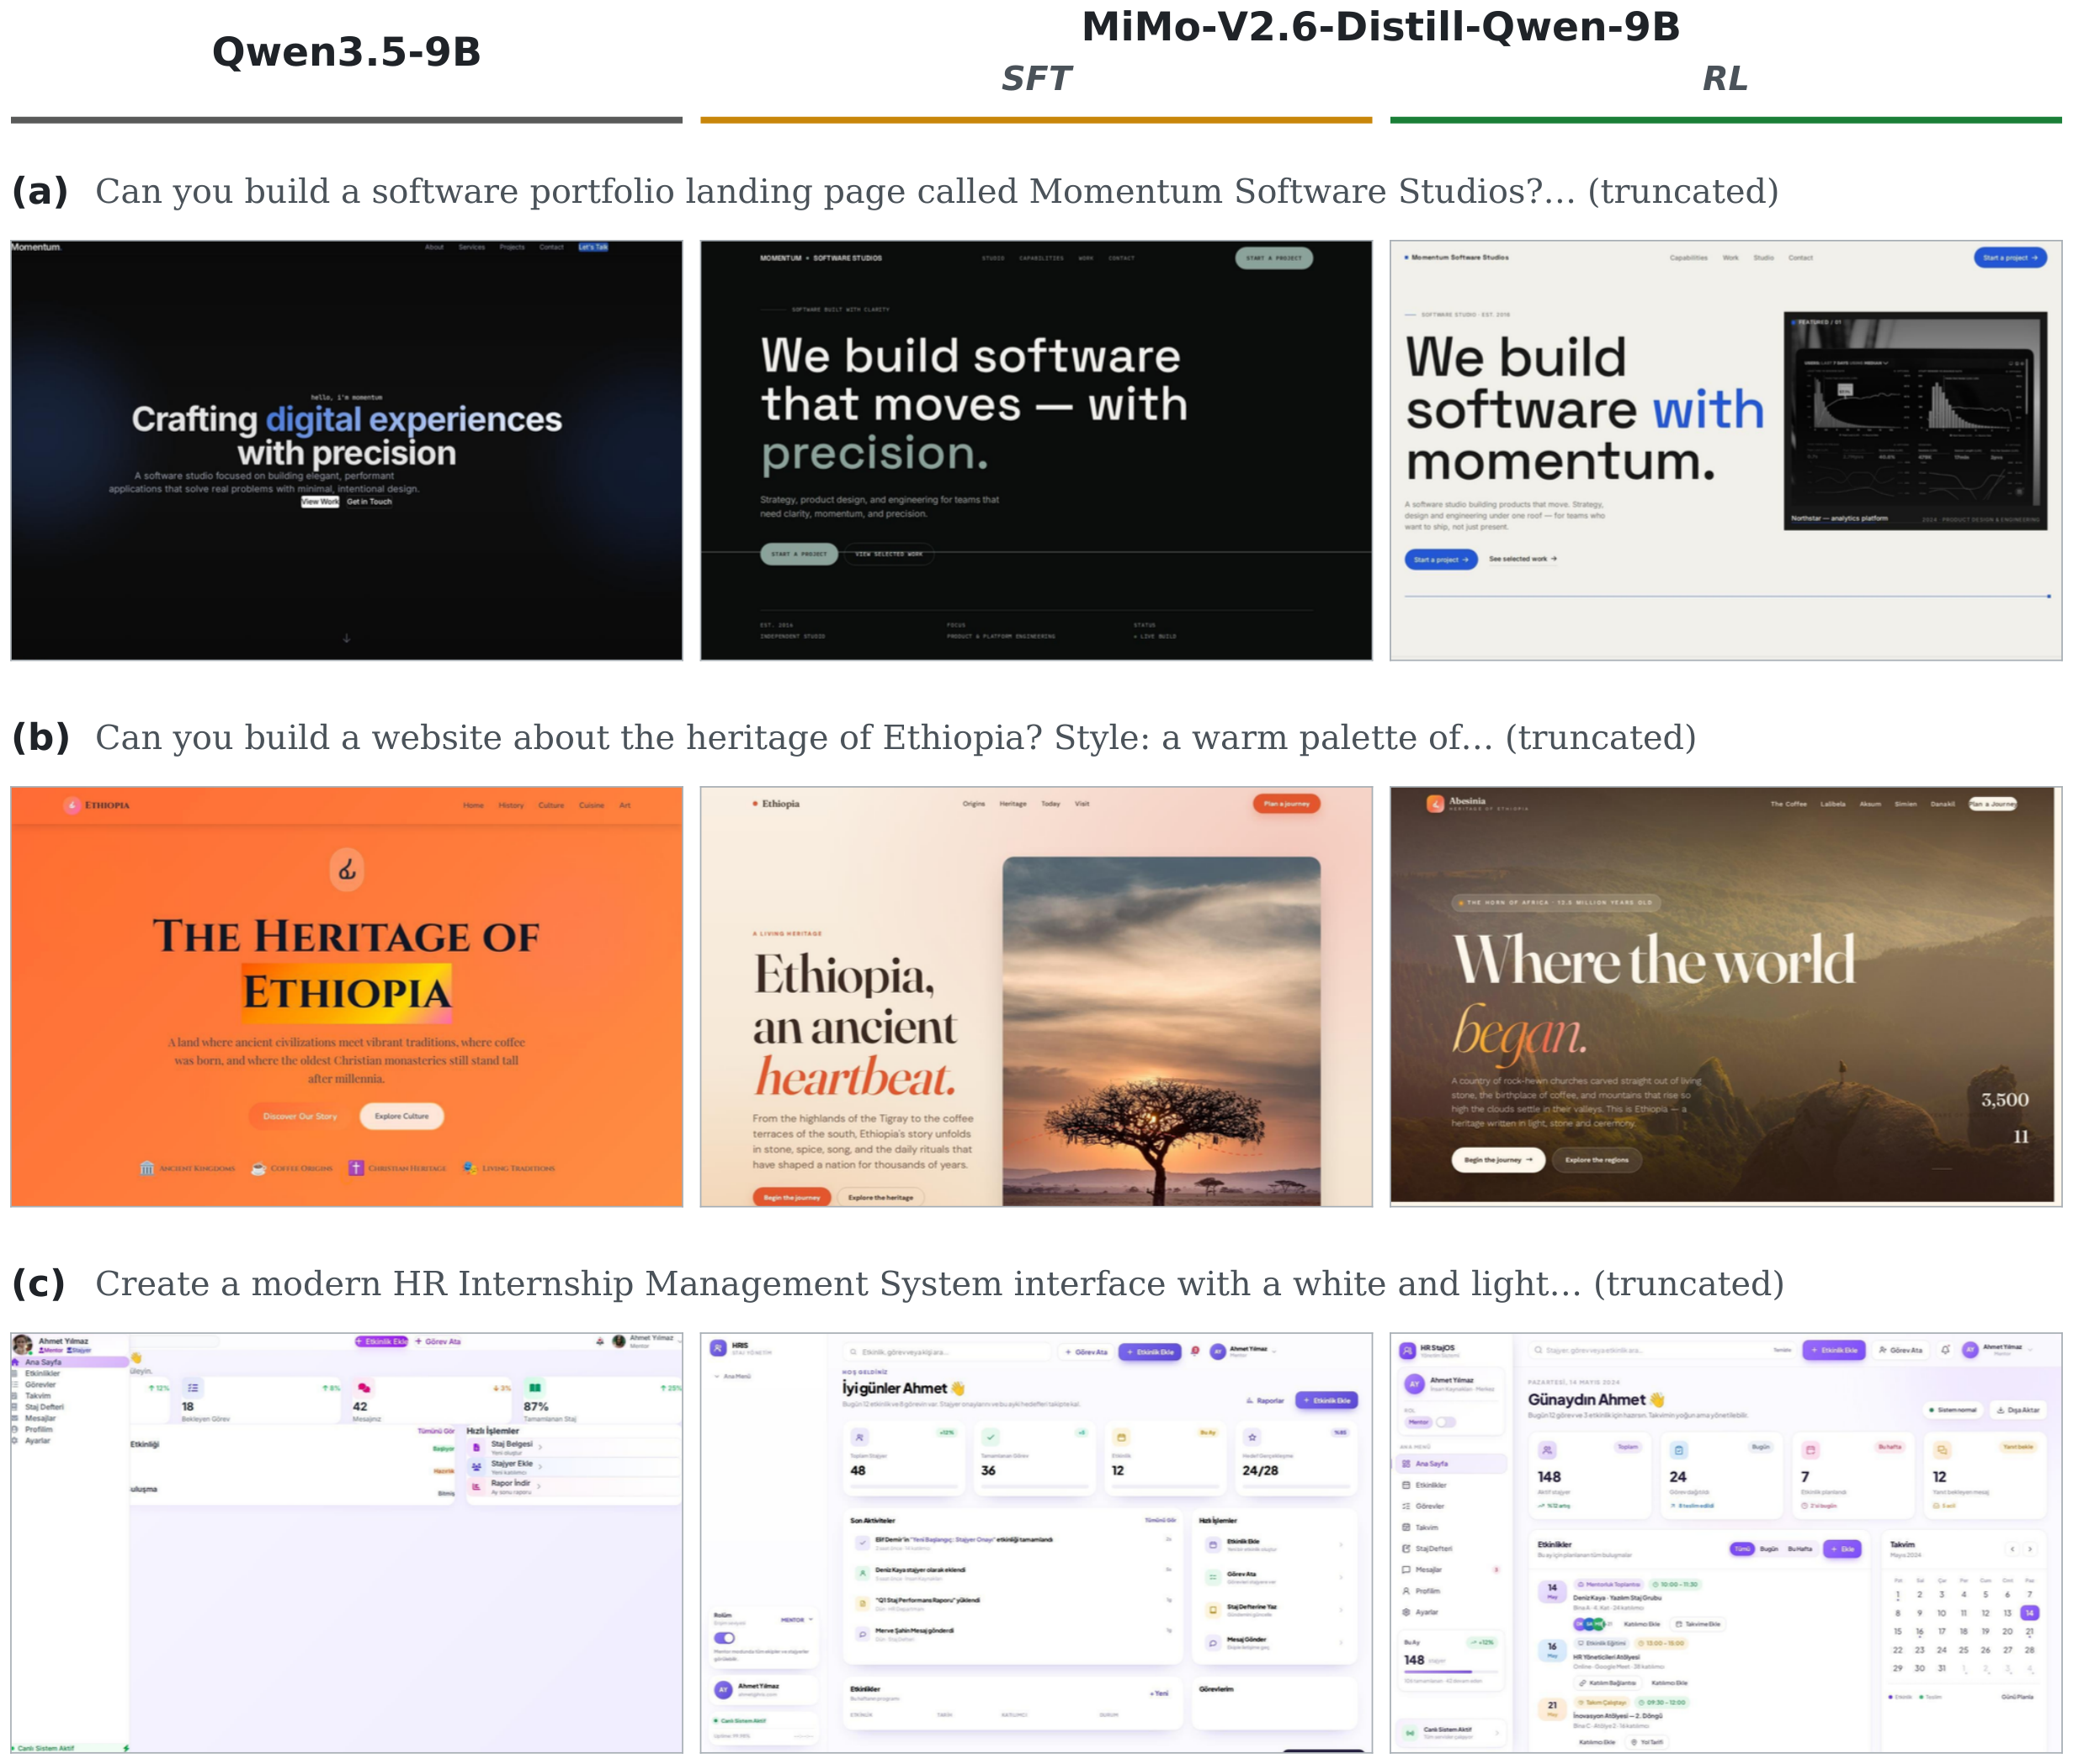
\includegraphics[width=\linewidth]{images_hi/fig17.png}
\caption{由 Qwen3.5-9B、MiMo-V2.6-Distill-Qwen-9B（SFT）和 MiMo-V2.6-Distill-Qwen-9B（RL）生成的网站首屏区域示例。每一行（a--c）展示三个模型对同一提示词的输出。}
\label{fig:17}
\end{figure}

\section*{参考文献}\label{references}

Artificial Analysis. GDPval-AA v2.1 Leaderboard, 2026. URL
https://artificialanalysis.ai/evalua tions/gdpval-aa. Accessed September
21, 2026.

I. Badertdinov, M. Nekrashevich, A. Shevtsov, and A. Golubev.
Swe-rebench v2: Languageagnostic swe task collection at scale, 2026. URL
https://arxiv.org/abs/2602.23866.

J. Chen, Y. Liang, and Z. Liu. Dflash: Block diffusion for flash
speculative decoding, 2026. URL https://arxiv.org/abs/2602.06036.

Core Team, B. Xiao, B. Xia, B. Yang, B. Gao, B. Shen, C. Zhang, C. He,
C. Lou, F. Luo, et al.~MiMo-V2-Flash technical report, 2026. URL
https://arxiv.org/abs/2601.02780.

X. Deng, J. Da, E. Pan, Y. Y. He, C. Ide, K. Garg, N. Lauffer, A. Park,
N. Pasari, C. Rane, et al.~Swe-bench pro: Can ai agents solve
long-horizon software engineering tasks?, 2025. URL
https://arxiv.org/abs/2509.16941.



F. Gloeckle, B. Y. Idrissi, B. Rozière, D. Lopez-Paz, and G. Synnaeve.
Better \& faster large language models via multi-token prediction. In
Forty-first International Conference on Machine Learning, ICML 2024,
Vienna, Austria, July 21-27, 2024. OpenReview.net, 2024. URL
https://openrevi ew.net/forum?id=pEWAcejiU2.

Z. Han, A. You, H. Wang, K. Luo, G. Yang, W. Shi, M. Chen, S. Zhang, Z.
Lan, C. Deng, et al.~Asyncflow: An asynchronous streaming rl framework
for efficient llm post-training, 2025. URL
https://arxiv.org/abs/2507.01663.

C. He, L. Li, S. Li, H. Lv, L. Kong, Q. Liu, T. Yang, and S. Ren.
Semantic head specialization guides hybrid vit attention for multimodal
llms, 2026. URL https://arxiv.org/abs/2608.28383.

HKUST NLP. Introducing Toolathlon-Verified, June 2026. URL
https://toolathlon.xyz/docs/bl og/toolathlon-verified.

W. Huang and P. Jiang. Deepswe v1.1: a cleaner, more reproducible
benchmark for frontier coding agents, 2026. URL
https://github.com/datacurve-ai/deep-swe.

W. Huang, C. Lee, L. Tng, and S. Ge. Deepswe: Measuring frontier coding
agents on original, long-horizon engineering tasks, 2026. URL
https://arxiv.org/abs/2607.07946.

C. E. Jimenez, J. Yang, A. Wettig, S. Yao, K. Pei, O. Press, and K. R.
Narasimhan. Swe-bench: Can language models resolve real-world github
issues? In The Twelfth International Conference on Learning
Representations, ICLR 2024, Vienna, Austria, May 7-11, 2024.
OpenReview.net, 2024. URL https://openreview.net/forum?id=VTF8yNQM66.

K. Jordan, Y. Jin, V. Boza, J. You, F. Cesista, L. Newhouse, and J.
Bernstein. Muon: An optimizer for hidden layers in neural networks,
2024. URL https://kellerjordan.github.io/posts/muon/.

Kimi Team. Kimi k1.5: Scaling reinforcement learning with llms, 2025.
URL https://arxiv.org/ abs/2501.12599.

H. Lee, J. Liu, D. Kim, Z. Zhang, C. S. Xia, and L. Zhang. Sec-bench
pro: Can language models solve long-horizon software security tasks?,
2026. URL https://arxiv.org/abs/2605.26548.

S. Lee and D. Brumley. Exploitbench: A capability ladder benchmark for
LLM cybersecurity agents, 2026. URL https://arxiv.org/abs/2605.14153.

J. Li, W. Zhao, J. Zhao, W. Zeng, H. Wu, X. Wang, R. Ge, Y. Cao, Y.
Huang, W. Liu, J. Liu, Z. Su, Y. Guo, F. Zhou, L. Zhang, J. Michelini,
X. Wang, X. Yue, S. Zhou, G. Neubig, and J. He. The tool decathlon:
Benchmarking language agents for diverse, realistic, and long-horizon
task execution. In International Conference on Learning Representations,
2026a. URL https://ar xiv.org/abs/2510.25726.

Y. Li, Y. Feng, Z. Xu, Z. Ma, K. Zheng, F. Jiang, X. Sun, R. Shao, Z.
Chen, Y. Huang, X. Han, B. Lee, K. Xu, S. Zeng, H. Hua, X. Zhang, B.
Alomair, R. Krishna, L. Zettlemoyer, P. W. Koh, B. Ramasubramanian, L.
Niu, X. Yue, and R. Poovendran. JobBench: Aligning agent work with human
will, 2026b. URL https://arxiv.org/abs/2605.26329.

B. Liao, H. Dong, C. Monz, X. Xu, L. Dong, and F. Wei. Multi-turn
on-policy distillation with prefix replay, 2026. URL
https://arxiv.org/abs/2607.04763.

K. Lion, F. Hübler, B. Li, A. Orvieto, and N. He. Muown: Row-norm
control for Muon optimization, 2026. URL
https://arxiv.org/abs/2605.10797.



A. Liu, B. Feng, B. Xue, B. Wang, B. Wu, C. Lu, C. Zhao, C. Deng, C.
Zhang, C. Ruan, et al.~Deepseek-v3 technical report, 2024. URL
https://arxiv.org/abs/2412.19437.

A. Liu, A. Mei, B. Lin, B. Xue, B. Wang, B. Xu, B. Wu, B. Zhang, C. Lin,
C. Dong, et al.~Deepseekv3.2: Pushing the frontier of open large
language models, 2025a. URL https://arxiv.org/abs/ 2512.02556.

J. Liu, J. Su, X. Yao, Z. Jiang, G. Lai, Y. Du, Y. Qin, W. Xu, E. Lu, J.
Yan, Y. Chen, H. Zheng, Y. Liu, S. Liu, B. Yin, W. He, H. Zhu, Y. Wang,
J. Wang, M. Dong, Z. Zhang, Y. Kang, H. Zhang, X. Xu, Y. Zhang, Y. Wu,
X. Zhou, and Z. Yang. Muon is scalable for LLM training, 2025b. URL
https://arxiv.org/abs/2502.16982.

W. Ma, H. Zhang, L. Zhao, Y. Song, Y. Wang, Z. Sui, and F. Luo.
Stabilizing moe reinforcement learning by aligning training and
inference routers, 2025. URL https://arxiv.org/abs/2510.1 1370.

W. Ma, J. Wei, L. Zhao, H. Zhang, B. Xiao, L. Li, Q. Yang, B. Gao, Y.
Wang, R. Li, J. Dong, Z. Sui, and F. Luo. Mopd: Multi-teacher on-policy
distillation for capability integration in llm posttraining, 2026. URL
https://arxiv.org/abs/2606.30406.

R. Marten, A. Shaw, I. Bercovich, B. Droste, T. Cerruti, S. Dillmann, R.
Wang, D. Wahdany, A. Hart, K. Krauth, ScaleAI, Snorkel AI, Turing,
gNucleus AI, Boolean AI, N. Carlini, S. Lyu, A. Wei, A. Khatua, B.
Plüster, C. Dwivedi, C. Sutcliffe, Yuming, D. Tivris, D. Wang, H. W. Goh,
H. Xing, H. Lin, I. Salia, J. Seol, J. Bao, J. Ouyang, J. Park, L.
Walsh, L. Kong, M. Ivanov, M. Ubl, M. Liamets, O. Menis, P. Migdal, Q.
Bao, R. Movva, R. Ben Chaim, N. Srinath, S. Bogdanik, S. Yadav, S.
Benjamin, T. Kung, W. Hughes, X. Lan, H. Gupta, S. Mishra, C. Wang, H.
He, J. Tu, K. Montgomery, Z. Tu, A. Naik, D. Mortensen, I. Zhang, Y.
Mathur, E. Liu, K. Singh, M. Yu, S. Feng, V. Gangal, Z. Tao, S. Ruan, J.
Mueller, J. Cabezas, J. Bauer, K. X. Li, R. Zhang, A. Feller, A.
Madayan, L. Chen, B. Feuer, X. Li, B. Li, H. Raj, S. Galler, L. Shi, I.
Segal, K. Buchanan, S. P., R. Desai, A. Schneider, C. Settles, X. Lin,
M. Nezhurina, A. Wang, M. Kowalczyk, J.-X. Zhao, S. Satia, J. Hu, S.
Atef, K. Chen, S. Vance, G. Segato, J. Jitsev, A. Dimakis, M. Merrill,
A. Konwinski, and L. Schmidt. Terminal-Bench, 2026. URL
https://github.com/harbor-framework/terminal-bench/releases/tag/v4.0.0.
Software release, version 4.0.0.

M. A. Merrill, A. G. Shaw, N. Carlini, B. Li, H. Raj, I. Bercovich, L.
Shi, J. Y. Shin, T. Walshe, E. K. Buchanan, J. Shen, G. Ye, H. Lin, J.
Poulos, M. Wang, M. Nezhurina, J. Jitsev, D. Lu, O. M. Mastromichalakis,
Z. Xu, Z. Chen, Y. Liu, R. Zhang, L. L. Chen, A. Kashyap, J.-L. Uslu, J.
Li, J. Wu, M. Yan, S. Bian, V. Sharma, K. Sun, S. Dillmann, A. Anand, A.
Lanpouthakoun, B. Koopah, C. Hu, E. Guha, G. H. S. Dreiman, J. Zhu, K.
Krauth, L. Zhong, N. Muennighoff, R. Amanfu, S. Tan, S. Pimpalgaonkar, T.
Aggarwal, X. Lin, X. Lan, X. Zhao, Y. Liang, Y. Wang, Z. Wang, C. Zhou,
D. Heineman, H. Liu, H. Trivedi, J. Yang, J. Lin, M. Shetty, M. Yang, N.
Omi, N. Raoof, S. Li, T. Y. Zhuo, W. Lin, Y. Dai, Y. Wang, W. Chai, S.
Zhou, D. Wahdany, Z. She, J. Hu, Z. Dong, Y. Zhu, S. Cui, A. Saiyed, A.
Kolbeinsson, J. Hu, C. M. Rytting, R. Marten, Y. Wang, A. Dimakis, A.
Konwinski, and L. Schmidt. Terminal-Bench: Benchmarking agents on hard,
realistic tasks in command line interfaces, 2026. URL
https://arxiv.org/abs/2601.11868.

P. Moritz, R. Nishihara, S. Wang, A. Tumanov, R. Liaw, E. Liang, M.
Elibol, Z. Yang, W. Paul, M. I. Jordan, et al.~Ray: A distributed
framework for emerging \{AI\} applications. In 13th USENIX symposium on
operating systems design and implementation (OSDI 18), pages 561--577,
2018.



K. Opsahl-Ong, A. Singhvi, J. Collins, I. Zhou, C. Wang, A. Baheti, O.
Oertell, J. Portes, S. Havens, E. Elsen, M. Bendersky, M. Zaharia, and
X. Chen. Officeqa pro: An enterprise benchmark for end-to-end grounded
reasoning, 2026. URL https://arxiv.org/abs/2603.08655.

T. Patwardhan, R. Dias, E. Proehl, G. Kim, M. Wang, O. Watkins, S. P.
Fishman, M. Aljubeh, P. Thacker, L. Fauconnet, N. S. Kim, P. Chao, S.
Miserendino, G. Chabot, D. Li, M. Sharman, A. Barr, A. Glaese, and J.
Tworek. GDPval: Evaluating AI model performance on real-world
economically valuable tasks, 2025. URL https://arxiv.org/abs/2510.04374.

PrimeIntellect. Swe-rl: Software engineering tasks for rl, 2026. URL
https://huggingface.co/col lections/PrimeIntellect/swe-rl.

X. Qu, P. Huang, and S. Horvath. Can Muon fine-tune Adam-pretrained
models?, 2026. URL https://arxiv.org/abs/2605.10468.

Qwen Team. Qwen3-next: Towards ultimate training \& inference efficiency.
https://qwen.ai/blog
?id=4074cca80393150c248e508aa62983f9cb7d27cd\&from=research.latest-advancements-list,
September 2025.

I. Shah, A. M. Polloreno, K. Stratos, P. Monk, A. Chaluvaraju, A. Hojel,
A. Ma, A. Thomas, A. Tanwer, D. J. Shah, K. Nguyen, K. Smith, M.
Callahan, M. Pust, M. Parmar, P. Rushton, P. Mazarakis, R. Kapila, S.
Srivastava, S. Singla, T. Romanski, Y. Vanjani, and A. Vaswani.
Practical efficiency of Muon for pretraining, 2025. URL
https://arxiv.org/abs/2505.02222.

Z. Shao, P. Wang, Q. Zhu, R. Xu, J. Song, X. Bi, H. Zhang, M. Zhang, Y.
K. Li, Y. Wu, and D. Guo. Deepseekmath: Pushing the limits of
mathematical reasoning in open language models, 2024. URL
https://arxiv.org/abs/2402.03300.

D. Shepard and R. Salimans. AutomationBench, 2026. URL
https://arxiv.org/abs/2604.18934.

M. Shoeybi, M. Patwary, R. Puri, P. LeGresley, J. Casper, and B.
Catanzaro. Megatron-lm: Training multi-billion parameter language models
using model parallelism, 2019. URL https://arxiv. org/abs/1909.08053.

Y. Sun, X. Han, W. Zhang, Y. Pang, T. Wang, Y. Cao, Y. Huang, C. Duroiu,
H. Zhang, J. Lin, W. Zhang, T. Zeng, Y. Yan, B. Liu, H. Wen, M. Xu, X.
Liu, Z. Chen, W. Shi, A. Dsouza, V. S. Chen, P. Bryant, C. Boettiger, Y.
Rangan, B. Rothenberg, K. Steinfeld, A. Rao, T. Schneider, G.
Yannakakis, L. Zanna, K. Ozbay, I. Sim, T. Zohdi, G. E. Karniadakis, J.
Gallant, T. Head-Gordon, Y. Li, W. Deng, T. Sun, H. Wang, Z. Wang, J.
Xu, C. Y. Liu, Y. Cheng, R. Hu, A. Bacho, S. Cao, Z. Qin, Y. Chen, H.
Fan, H. Liu, L. Zeng, S. M. Bharadwaj, L. Gong, Y. Yang, M. Song, R.
Wang, Z. Zhang, H. Bao, S. Lu, J. Tu, Z. Wang, Z. Zhang, Z. Chen, Y.
Jiang, Z. Li, B. Lyu, C. Ma, P. Xu, B. Zhang, S. Gu, H. Hua, H. Li, W.
Liao, C. Liu, J. Peng, H. Sun, Z. Xu, B. Chen, J. Cheng, Y. Jiang, K.
Kuang, Y. Li, Y. Pan, Z. Rao, A. Schubert, Y. Shen, V. Siu, X. Sun, K.
Zhang, X. Zhang, Y. Zhu, I. S. Chandok, L. Ding, J. Fan, A. Glover, J.
Hu, Y. Hu, W. Huang, Z. Jiang, H. Jin, L. Kim, M. Liu, Y. Liu, A.
Rafiei, X. Shen, K. Sun, S. Sun, T. Sun, E. Wang, Y. Wang, H. Xing, S.
Xu, Y. Xu, Z. Xu, Z. Yan, B. Yuan, R. Zhang, Y. Zhang, Z. Zhao, Liana,
S. B. Antu, H. Bai, C. Bosio, J. Cavanagh, P. Cavazos-Rehg, T. Chen, X.
Chen, Y. Chen, C. Zhu, C. Dai, S. D. Castro, Y. Deng, K. Dhole, J. Ding,
C. Du, Z. Du, H. Fan, R.-Z. Fan, H. Fu, S. Gu, Y. Gu, C. Guo, B. Huang,
B. Huang, R. Jaiswal, Z. Jiang, R. Jin, E. Kasson, X. Lan, J. Lee, D.
Lei, C. Li, D. Li, H. Li, H. Li, J. Li, X. Li, Y. Li, Y. Li, Y. Li, Z.
Li, W. Liang, L. Liao, K. Q. Lin, A. Z. Liu, C. Liu, J. Liu, K. Liu, X.
Liu, P. Lu, W. Lv, Y. Lyu, Q. Mang, K. Montgomery, Y. Nie, R. Ning, J.
Overwiening, X. Pan, L. Paraboschi, C. F. Park, J. Purnomo, S. Rajwal,
S. Rankin, B. Ren, Y. Rong, H. Shang, V. Shaw, F. Shen, J. Shen, M. Shi,
S. Qiu, H. Yao, T. Shi, J. So, V. Susoy, H. Szlyk, H. Wang,



J. Wang, W. Wang, X. Wang, Z. Wang, D. Wong, A. Wu, D. Wu, F. Wu, M. M.
Wu, Y. Wu, Y. Wu, Y. Wu, Q. Wuwu, W. Xiao, Y. Xiong, F. Xu, R. Xu, M.
Yan, B. Yang, J. Yang, S. Yang, X. Yang, Y. Yang, H. Ye, X. Yu, Z. Yu,
C. Zhang, C. Zhang, H. Zhang, H. Zhang, J. Zhang, K. Zhang, S. Zhang, W.
Zhang, W. Zhang, Y. Zhang, Y. Zhang, B. Zhao, Q. Zhao, Y. Zhao, Y.
Zheng, L. Zhou, T. Zhou, S. Zhu, S. Zhu, Y. Zhu, Y. Zhu, J. Zuo, C. Cai,
H. Casademunt, W. Chen, C. Cheng, N. Deng, R. Fu, T. Fu, Y. Han, H. Ren,
Z. He, Q. Jin, L. Li, Y. Li, S. Liu, L. Lu, L. Zhou, S. Mukherjee, Y.
Ouyang, Y. Ren, D. Shi, H. Wu, Z. Wu, H. Yao, Z. Yi, J. Yu, R. Zhan, H.
Zhou, B. Zhu, J. Zhu, A. Yuille, Y. Liu, R. A. Poldrack, J. Li, Z. Li,
M. Tao, J. Huang, W. Shi, C. Spanos, L. Sun, C. Wang, O. Xu, Z. Dong, H.
Gomez, A. Caliskan, A. Emami, H. Hu, Z. Li, L. Liu, M. Niu, Y. Shao, J.
Sun, M. Tolonen, T. Wang, S. Das, Y. Gao, W. Guo, E. J. Schneider, Z.
Lu, Y. Ma, M. Mueller, R. Poovendran, S. Sojoudi, Y. Zhu, and D. Song.
Agents' last exam, 2026. URL https://arxiv.org/abs/2606.05405.

C. Tao, J. Chen, Y. Jiang, K. Kou, S. Wang, R. Wang, X. Li, S. Yang, Y.
Du, J. Dai, Z. Mao, X. Wang, L. Shang, and H. Bai. Swe-lego: Pushing the
limits of supervised fine-tuning for software issue resolving, 2026. URL
https://arxiv.org/abs/2601.01426.

The Microsoft AI Team. MAI-Thinking-1: Building a hill-climbing machine.
Technical report, Microsoft AI, 2026. URL
https://microsoft.ai/pdf/mai-thinking-1.pdf.

A. Vaswani, N. Shazeer, N. Parmar, J. Uszkoreit, L. Jones, A. N. Gomez,
L. Kaiser, and I. Polosukhin. Attention is all you need. In I. Guyon, U.
von Luxburg, S. Bengio, H. M. Wallach, R. Fergus, S. V. N. Vishwanathan,
and R. Garnett, editors, Advances in Neural Information Processing
Systems 30: Annual Conference on Neural Information Processing Systems
2017, December 4-9, 2017, Long Beach, CA, USA, pages 5998--6008, 2017.
URL https://proceedings.neurips.
cc/paper/2017/hash/3f5ee243547dee91fbd053c1c4a845aa-Abstract.html.

vLLM Project. Humming. https://github.com/vllm-project/humming/releases/tag/v0.1.15,
September 2026. Version 0.1.15, GitHub repository, commit
a74973b5079e42ef861720b62f847ce9d33447f5; accessed 2026-09-19.

Z. Wang, T. Shi, J. He, M. Cai, J. Zhang, and D. Song. Cybergym:
Evaluating AI agents' cybersecurity capabilities with real-world
vulnerabilities at scale, 2025. URL https://arxiv.org/abs/ 2506.02548.

Z. Wang, N. Schiller, H. Li, S. S. Narayana, M. Nasr, N. Carlini, X. Qi,
E. Wallace, E. Bursztein, L. Invernizzi, K. Thomas, Y. Shoshitaishvili,
W. Guo, J. He, T. Holz, and D. Song. Exploitgym: Can AI agents turn
security vulnerabilities into real attacks?, 2026. URL
https://arxiv.org/ab s/2605.11086.

B. Xia, B. Shen, D. Zhu, D. Zhang, G. Wang, H. Zhang, H. Liu, J. Xiao,
J. Dong, L. Zhao, et al.~Mimo: Unlocking the reasoning potential of
language model--from pretraining to posttraining, 2025. URL
https://arxiv.org/abs/2505.07608.

L. Xiaomi. Mimo-audio: Audio language models are few-shot learners,
2025. URL https://arxiv. org/abs/2512.23808.

T. Xie, D. Zhang, J. Chen, X. Li, S. Zhao, R. Cao, T. J. Hua, Z. Cheng,
D. Shin, F. Lei, Y. Liu, Y. Xu, S. Zhou, S. Savarese, C. Xiong, V.
Zhong, and T. Yu. Osworld: Benchmarking multimodal agents for open-ended
tasks in real computer environments. In A. Globersons, L. Mackey, D.
Belgrave, A. Fan, U. Paquet, J. M. Tomczak, and C. Zhang, editors,
Advances in Neural Information Processing Systems 37: Annual Conference
on Neural Information Processing Systems 2024, NeurIPS 2024, Vancouver,
BC, Canada, December 10 - 15, 2024, 2024. doi: 10.52202/07901



7-1650. URL
http://papers.nips.cc/paper\_files/paper/2024/hash/5d413e48f84dc61244b6be5
50f1cd8f5-Abstract-Datasets\_and\_Benchmarks\_Track.html.

XLANG Lab. Introducing OSWorld-Verified, July 2025. URL
https://xlang.ai/blog/osworld-verif ied.

W. Xu, R. Han, Z. Wang, L. T. Le, D. Madeka, L. Li, W. Y. Wang, R.
Agarwal, C. Lee, and T. Pfister. Speculative knowledge distillation:
Bridging the teacher-student gap through interleaved sampling. In The
Thirteenth International Conference on Learning Representations, ICLR
2025, Singapore, April 24-28, 2025. OpenReview.net, 2025. URL
https://openreview.net/forum?i d=EgJhwYR2tB.

J. Yang, K. Lieret, J. Ma, P. Thakkar, D. Pedchenko, S. Sootla, E.
McMilin, P. Yin, R. Hou, G. Synnaeve, D. Yang, and O. Press.
Programbench: Can language models rebuild programs from scratch?, 2026a.
URL https://arxiv.org/abs/2605.03546.

S. Yang, C. Tao, J. Chen, T. Yu, R. Wang, Y. Jiang, Y. Du, W. Xu, J.
Xiong, T. Wu, L. Shang, X. Li, N. Wong, and H. Bai. What makes
interaction trajectories effective for training terminal agents?, 2026b.
URL https://arxiv.org/abs/2606.03461.

B. Ye, L. Li, S. Li, Z. Yue, L. Zhang, H. Lv, Y. Liu, W. Ma, H. Tian, R.
Li, J. Dong, Y. Zhao, X. Deng, H. Zhang, L. Zhao, Q. Liu, L. Kong, T.
Yang, and F. Luo. CodeMidas: Scaling agentic coding rl environments from
code itself, 2026. URL https://arxiv.org/abs/2609.22068.

Q. Yu, Z. Zhang, R. Zhu, Y. Yuan, X. Zuo, Y. Yue, W. Dai, T. Fan, G.
Liu, J. Liu, L. Liu, X. Liu, H. Lin, Z. Lin, B. Ma, G. Sheng, Y. Tong,
C. Zhang, M. Zhang, R. Zhang, W. Zhang, H. Zhu, J. Zhu, J. Chen, J.
Chen, C. Wang, H. Yu, Y. Song, X. Wei, H. Zhou, J. Liu, W. Ma, Y. Zhang,
L. Yan, Y. Wu, and M. Wang. DAPO: an open-source LLM reinforcement
learning system at scale. In D. Belgrave, C. Zhang, L. N. Montoya, H.
Lin, R. Pascanu, P. Koniusz, M. Ghassemi, N. Chen, I. V. M. Ruíz, and A.
Loaiza-Bonilla, editors, Advances in Neural Information Processing
Systems 38: Annual Conference on Neural Information Processing Systems
2025, NeurIPS 2025, San Diego, CA, USA, December 2-7, 2025 / Mexico
City, Mexico, November 30 - December 5, 2025, 2025. URL
http://papers.nips.cc/paper\_files/paper/2025/hash/a4277
440d50f1f15d2cb4c14f7e0c0d2-Abstract-Conference.html.

Z. Yue, Z. Lin, Y. Song, W. Wang, S. Ren, S. Gu, S. Li, P. Li, L. Zhao,
L. Li, et al.~Mimo-vl technical report, 2025. URL
https://arxiv.org/abs/2506.03569.

D. Zan, Z. Huang, W. Liu, H. Chen, S. Xin, L. Zhang, Q. Liu, A. Li, L.
Chen, X. Zhong, S. Liu, Y. Xiao, L. Chen, Y. Zhang, J. Su, T. Liu, R.
Long, M. Ding, and L. Xiang. Multi-swebench: A multilingual benchmark
for issue resolving. In D. Belgrave, C. Zhang, L. N. Montoya, H. Lin, R.
Pascanu, P. Koniusz, M. Ghassemi, N. Chen, I. V. M. Ruíz, and A.
Loaiza-Bonilla, editors, Advances in Neural Information Processing
Systems 38: Annual Conference on Neural Information Processing Systems
2025, NeurIPS 2025, San Diego, CA, USA, December 2-7, 2025 / Mexico
City, Mexico, November 30 - December 5, 2025, 2025. URL http:
//papers.nips.cc/paper\_files/paper/2025/hash/5afa9cb1e917b898ad418216dc726fbd-A
bstract-Datasets\_and\_Benchmarks\_Track.html.

J. Zhao, G. Chen, F. Meng, M. Li, J. Chen, H. Xu, Y. Sun, X. Zhao, R.
Song, Y. Zhang, P. Wang, C. Chen, J. Wen, and K. Jia. Immersion in the
github universe: Scaling coding agents to mastery, 2026. URL
https://arxiv.org/abs/2602.09892.



L. Zheng, L. Yin, Z. Xie, C. Sun, J. Huang, C. H. Yu, S. Cao, C.
Kozyrakis, I. Stoica, J. E. Gonzalez, C. W. Barrett, and Y. Sheng.
Sglang: Efficient execution of structured language model programs. In A.
Globersons, L. Mackey, D. Belgrave, A. Fan, U. Paquet, J. M. Tomczak,
and C. Zhang, editors, Advances in Neural Information Processing Systems
37: Annual Conference on Neural Information Processing Systems 2024,
NeurIPS 2024, Vancouver, BC, Canada, December 10 - 15, 2024, 2024. URL
http://papers.nips.cc/paper\_files/paper/2024/hash/724be4472168f31
ba1c9ac630f15dec8-Abstract-Conference.html.

\section{贡献与致谢}\label{a-contributions-and-acknowledgments}

我们衷心感谢所有贡献者给予的宝贵支持与付出，包括 Xiaomi Data Platform、
CloudML、NGK、MiChat、Mify、MiKS 和 LLM-Plus 团队，以及本文未明确列出的各位。
在每个角色内部，作者按名字首字母的逆序排列。

核心贡献者：Zongming Qiao, Ziyue Hua, Zirui Ou, Zihao Yue, Zihan
Jiang, Zhuo Huang, Zhiyang Chen, Zhixian Zheng, Zhipeng Xu, Zhengrui Ma,
Yuyang Hu, Yuhang Dong, Yuechen Zhang, Yudong Wang, Yuanxin Liu, Yixin
Yang, Yishuo Cai, Yikai Zhao, Yihan Yan, Yifan Zhang, Yifan Song, Xiyu
Wei, Xing Zhang, Xin Zhang, Xiaoqian Liu, Xiaodong Ji, Xiangwei Deng,
Xueyu Guo, Wenhan Ma, Weimin Xiong, Weikun Wang, Weiji Zhuang, Shuo Liu,
Shuhuai Ren, Shuhao Gu, Shimao Chen, Shijie Cao, Shihua Yu, Shicheng Li,
Shengjie Zhou, Shaolei Zhang, Rang Li, Qiying Wang, Qingkai Fang, Qianli
Chen, Minzheng Wang, Liwen Wang, Linli Yao, Linghao Zhang, Liangyu
Cheng, Liang Zhao, Lei Li, Jinhao Dong, Jinyu Xiang, Jianyu Wei,
Jiangshan Duo, Huaqiu Liu, Huanjie Fan, Hongyi Guan, Hongshen Xu, Hao
Tian, Hanyu Li, Hailin Zhang, Gang Wang, Fuli Luo†, Feng Wei, Dong
Zhang, Dawei Zhu, Chiheng Lou, Chenhong He, Chenhao He, Chenghua Liu,
Bowen Ye, Bowen Shen, Boshen Xu, Bo Yang, Bingquan Xia, Bangjun Xiao,
Baixuan Xu

贡献者：Zhouxiang Mao, Zhiyang Zhang, Zhixiang Xu, Zhenru Lin,
Zhengju Tang, Zhaojun Huang, Yuzhe Weng, Yuxing Xiang, Yuxiao Li, Yuheng
Yang, Yuhang Wang, Yuchen Liu, Yuanyuan Tian, Yuanliang Dong, Yu Cheng,
Yongzhe He, Yongshun Liang, Yong Wang, Yiyan Wang, Yitian Gong, Yijie
Zhang, Yanshu Xin, Xun Zhang, Xingjian Zhao, Wenyu Yang, Wenshan Huang,
Wenhao Li, Tingwei Huang, Tianyu Yu, Tianyang Lu, Taoyu Yang, Sinan Du,
Shutong Tian, Shulin Du, Shengfan Wang, Shanchuan Fang, Qihao Zhang,
Qibin Yang, Qian Yu, Qian Tu, Pengrong Xie, Peipei Wang, Peidian Li,
Minkun Guo, Mingchen Shao, Luohan Gao, Lijie Wang, Liang Shi, Kaiqi
Chen, Kaiming Liu, Kaifei Wang, Kai Yang, Jinlong Xue, Jiechen Zhang,
Jiaxuan Liu, Hongxu An, Hao Peng, Hanglong Lü, Guonan Wang, Feiyu Yang,
Fanyu Cao, Fangyue Liu, Fan Cui, Cong Wang, Chun Chen, Chenxu Bai,
Chengxuan Zhu, Chenghua Wang, Boyi Zeng

†通讯作者

\end{document}
